%http://www.feradz.com/How_to_Write_Thesis.html
%Matici sa staruju len aby predali spravnost, Informatici aj motivaciu.

%Semantika 
%TODO final read thru
%TODO equation numbers only if I use them
%TODO ref as citations 
%TODO citet, citep
%TODO minimize itemize 
%TODO spellcheck 

%Stylistika: 
%TODO obojstranne 
%TODO check figures, tables, equations, algorithms 
%TODO check bibliography 
%TODO testing preprint (my version) 
%TODO 4-5 riadkov na jeden odstavec 
%TODO reread + tilde before (after i.e., before \ref, after short words... 
%TODO LaTeX warnings 
%TODO empty pages 

%TODO resolve TODO 

\documentclass[12pt,a4paper]{article}

\usepackage[utf8]{inputenc}
\usepackage{a4wide}
\usepackage{tabularx}
\usepackage{amsfonts}
\usepackage{amssymb}
\usepackage{amsmath}
\usepackage{epsfig}
\usepackage{color}
\usepackage{mathrsfs}
\usepackage{verbatim}
\usepackage{hyperref}
\usepackage{subfigure}
\usepackage{float}
\usepackage{longtable}

\usepackage[section]{algorithm}
\usepackage[]{algorithmicx}
\usepackage{algpseudocode}

\usepackage{multicol}
\usepackage{graphicx}
\usepackage{pdfpages}
\usepackage{lastpage}
\usepackage{fancyhdr}
\usepackage{url}
\usepackage[small,bf]{caption}
\usepackage{csquotes}  
\usepackage[T1]{fontenc}   

\usepackage{apalike}
\let\bibhang\relax
\usepackage[authoryear]{natbib}

%\newcommand{\quotes}[1]{``#1''}
                                  
\hypersetup{%  http://www.tug.org/applications/hyperref/
    bookmarksnumbered,
    pdfstartview={FitH},
    %linkcolor=black,
    %citecolor=black,
    colorlinks=true
}

\let\stdsection\section{}
\renewcommand\section{\newpage\stdsection}

%%%%%%%%%%%%%%%%%%%%%%%%% CUSTOMIZACIA BEGIN %%%%%%%%%%%%%%%
\setlength{\textheight}{24cm}
\setlength{\textwidth}{15.5cm}
\addtolength{\voffset}{-1.2cm}
\addtolength{\hoffset}{0.0cm}
\setlength{\parindent}{0.5cm}
\setlength{\parskip}{0in}
\setlength{\headheight}{16pt}
\linespread{1.5}

\hypersetup{
    colorlinks=true,       % false: boxed links; true: colored links
%    linkcolor=black,          % color of internal links
    citecolor=blue,        % color of links to bibliography
%    urlcolor=black,           % color of external links
%    linkbordercolor=black, % 	color of frame around internal links (if colorlinks=false)
%    citebordercolor=black, %	color of frame around citations
%    urlbordercolor=black, %	color of frame around URL links
}

%\setlength{\topmargin}{-10mm}
%\setlength{\textwidth}{16truecm}
%\setlength{\textheight}{24truecm}
%\setlength{\oddsidemargin}{0mm}
%\setlength{\evensidemargin}{0mm}
%%%%%%%%%%%%%%%%%%%%%%%%% CUSTOMIZACIA END %%%%%%%%%%%%%%%

\begin{document}

% ==================== 0. Cover ========================
\setcounter{page}{1}
\pagenumbering{roman}
\thispagestyle{empty}

    \begin{center}
    \large{
        \textbf{
            UNIVERZITA KOMENSKÉHO V BRATISLAVE \\ 
            FAKULTA MATEMATIKY, FYZIKY A INFORMATIKY
        }
    }
\end{center}

\vspace{2cm}

\begin{figure}[!h]
    \centering
    
\includegraphics[width=3.5cm]{img/komlogo-new}
\end{figure}

\vspace{1cm}

\begin{center}
    \large{
        \textbf{
            ANALYSIS OF THE GENERALIZED \\
            RECIRCULATION-BASED LEARNING ALGORITHM \\
            IN BIDIRECTIONAL NEURAL NETWORK \\
            \vspace{3cm}
            DIPLOMA THESIS
        }
    }
\end{center}

\vfill

\begin{multicols}{2}
    \begin{flushleft}
        \textbf{Bratislava 2014}
    \end{flushleft}
    \begin{flushright}
        \textbf{Bc. Peter CSIBA}
    \end{flushright}
\end{multicols}

    
% ==================== 1. Title ========================
%You should be very careful choosing a title for your thesis. It should exactly describe what your thesis is about. You should avoid long title because it is difficult to remember. Also the title shouldn’t be too short and mention just about a general problem or a field. Example title might be “Dynamic Thread Scheduling in Heterogeneous Multi Processors” or “Static Analysis for Unprotected Concurrent Memory Accesses” or “Detecting and Executing Parallel Code in GPUs”.
%\newpage
%\thispagestyle{empty}
%\addtolength{\hoffset}{4mm}
%\setlength{\oddsidemargin}{-5mm}
%\setlength{\evensidemargin}{5mm}

%    \begin{center}
    \large{
        \textbf{
            UNIVERZITA KOMENSKÉHO V BRATISLAVE \\ 
            FAKULTA MATEMATIKY, FYZIKY A INFORMATIKY
        }
    }
\end{center}

\vspace{2cm}

\begin{figure}[!h]
    \centering
    
\includegraphics[width=3.5cm]{img/komlogo-new}
\end{figure}

\vspace{1cm}

%TODO slovensky nazov 
\begin{center}
    \large{
        \textbf{
            ANALYSIS OF THE GENERALIZED \\
            RECIRCULATION-BASED LEARNING ALGORITHM \\
            IN BIDIRECTIONAL NEURAL NETWORK \\
            \vspace{3cm}
            DIPLOMOVÁ PRÁCA
        }
    }
\end{center}

\vfill

\begin{multicols}{2}
    \begin{flushleft}
        \textbf{Bratislava 2014}
    \end{flushleft}
    \begin{flushright}
        \textbf{Bc. Peter CSIBA}
    \end{flushright}
\end{multicols}



    
% ==================== 1+. Assignment ========================
\newpage

    
\thispagestyle{empty}
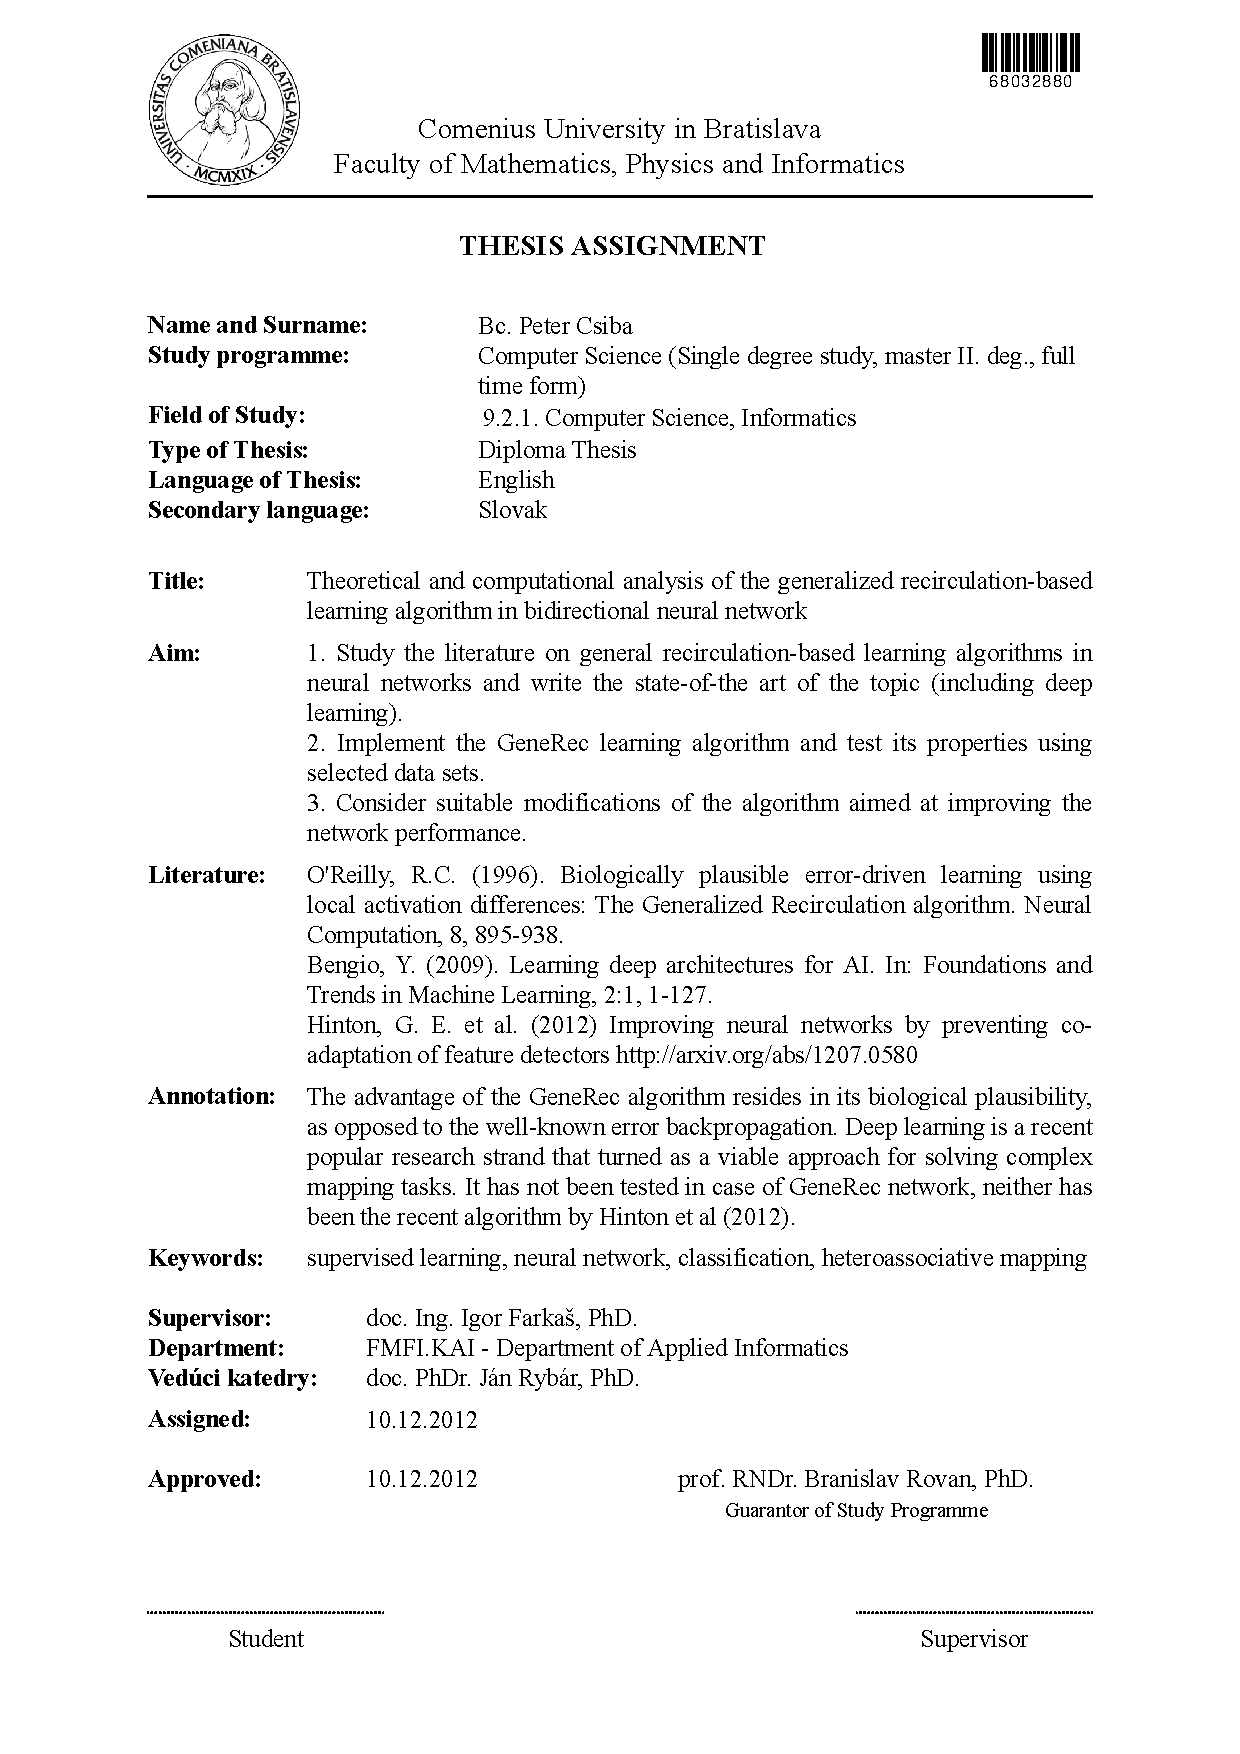
\includepdf[offset=0 -25mm]{img/zadanie-en.pdf}

\cleardoublepage
\thispagestyle{empty}
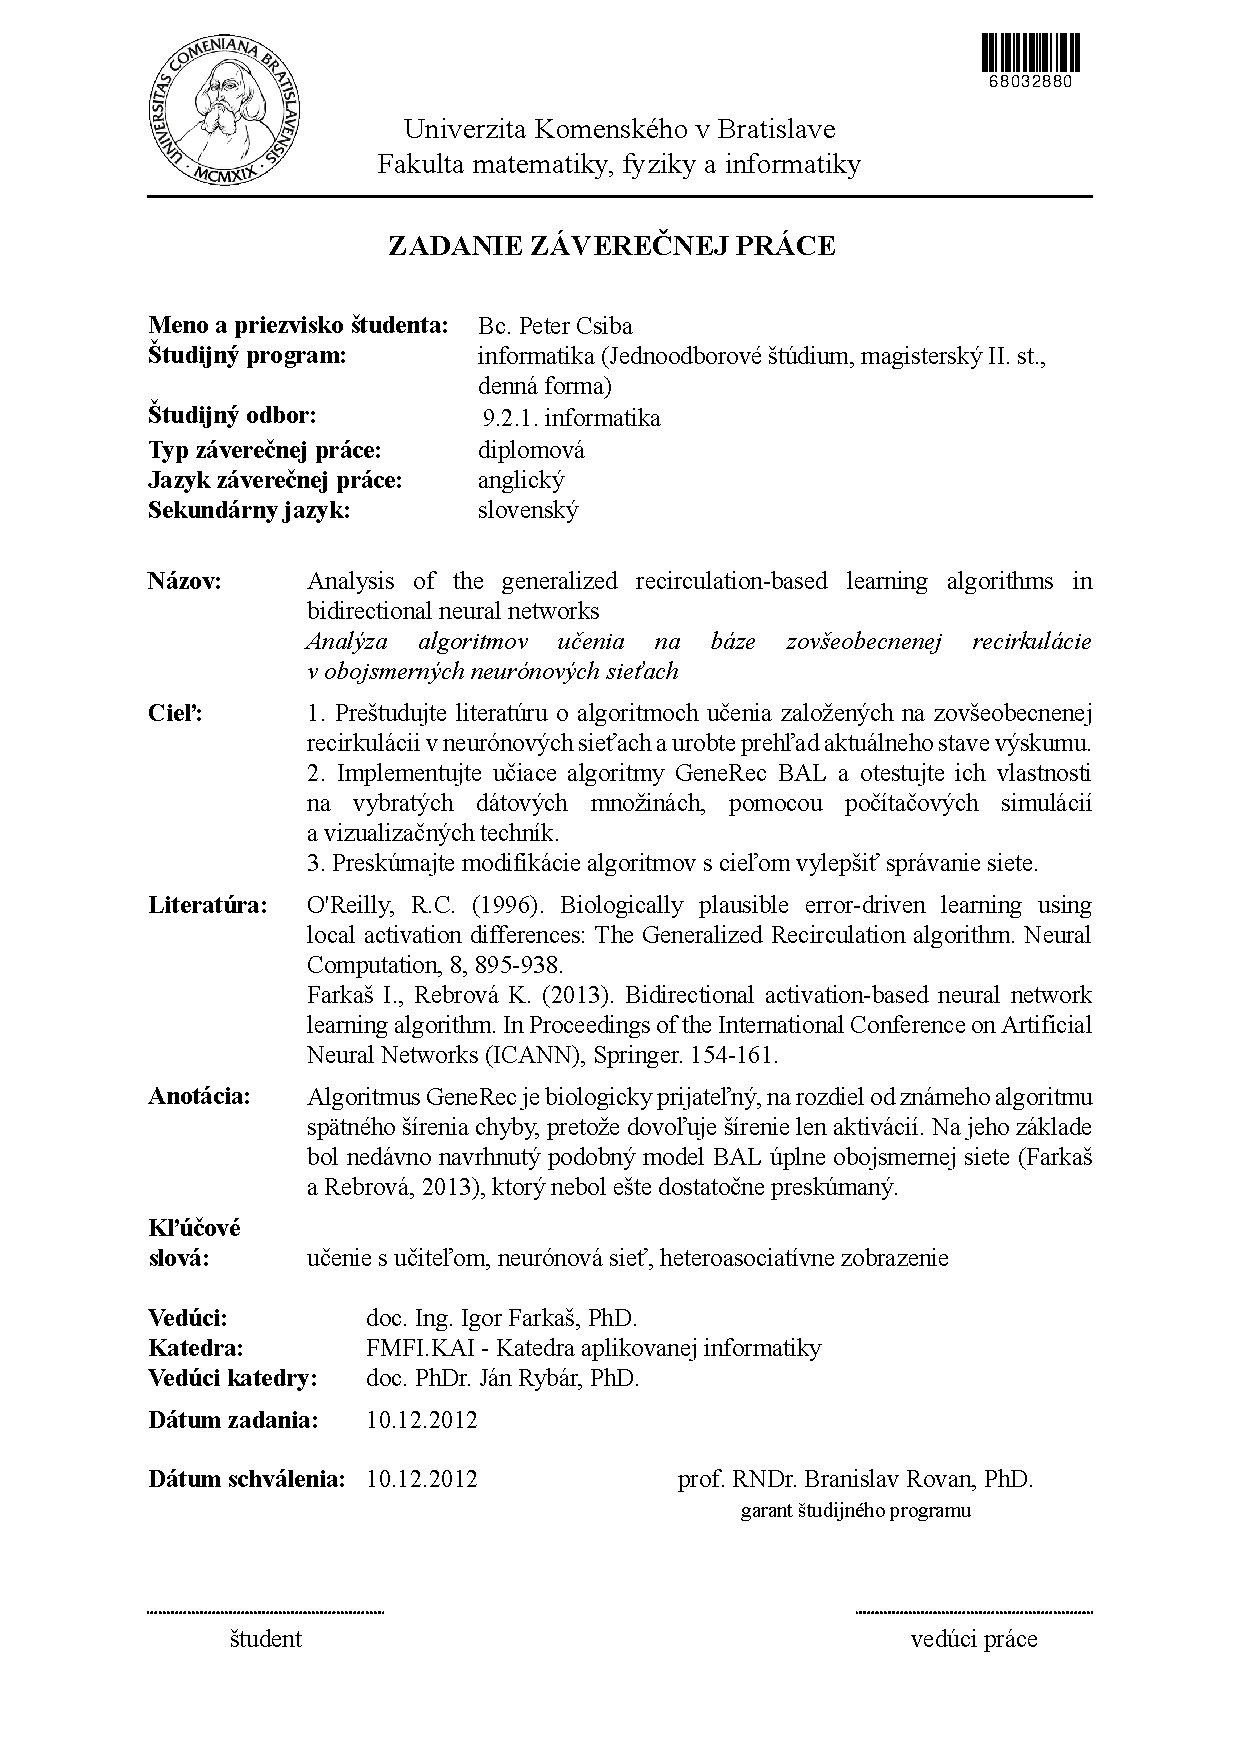
\includepdf[offset=0 -25mm]{img/zadanie-sk.pdf}


% ==================== 2. Dedication ========================
% Write to whom you dedicate you thesis if any. For example “I would like to dedicate this thesis to my mother and father…”
\newpage
%\thispagestyle{empty}
\thispagestyle{plain}

    %Write to whom you dedicate you thesis if any. For example “I would like to dedicate this thesis to my mother and father…”



% ==================== 3. Acknowledgements ========================
%It’s good to acknowledge the people who helped or participated in direct or indirect way to your thesis. Here is the place to thank to your supervisor and colleagues.
\newpage
%\thispagestyle{empty}
\thispagestyle{plain}

    % ==================== 3. Acknowledgements ========================
%It’s good to acknowledge the people who helped or participated in direct or indirect way to your thesis. Here is the place to thank to your supervisor and colleagues.

\null 
\vfill 

\subsection*{Acknowledgements}

The completion of this thesis could not have been possible without my supervisor Igor Farkaš who encouraged and helped me out through the whole process. Especially, I want to thank him for investing his precious time in our weekly sessions which navigated me what to do next and made me work regularly. 

I alsow want to thank my parents Viktor and Jarmila for their lifelong investement for providing me with the best education they could while often sacrifing their own comfort. 


% ==================== 4. Abstract  ========================
%Abstract is very important part of the thesis. It will be most read by people and should be written with a great care. The abstract should mention:

\newpage
%\thispagestyle{empty}

    %Abstract is very important part of the thesis. It will be most read by people and should be written with a great care. The abstract should mention:
% 1) About the problem you want to solve
% 2) About your solution – how you solve the problem
% 3) Highlights about how good is your solution (e.g. achieves 70\% better performance) referring to the results you obtained in your experiments (e.g. achieves 70\% better performance).
% 4) Possible impacts of your work into the field (e.g. “The proposed solution can be used to offload the CPU by executing data parallel computation intensive code on GPUs and thus obtaining additional Speedup for no cost”).

\section*{Abstract}

% 1) About the problem you want to solve
In our work, we used computational simulations to analyse supervised artificial neural networks based on the Generalized recirculation algorithm (GeneRec) by~\citet{o1996bio} and the Bidirectional Activation-based Learning algorithm (BAL) by~\citet{farkas2013bal}. The main idea of both algorithms is to update weights based on the difference between forward and backward propagation of neuron activations rather than based on error backpropagation (BP) between layers, which is considered biologically implausible. However, both algorithms struggle to learn low dimensional mappings which could be easily learned by BP. The aim of this work is to fill this gap. 

% 2) About your solution – how you solve the problem
Several modifications of BAL are proposed and after systematic analysis a Two learning rates (TLR) version is introduced. TLR uses different learning rates for different weight matrices. The simulations prove increase in success rate and show smooth relation between success and learning rates. For the networks with highest success rate the two learning rates can be in ratio $10^6$. Further the idea of TLR is applied to GeneRec. Finally, additional experiments for momentum, weight initialization, hidden activations and dynamic learning rate are analysed. 

% 4) Possible impacts of your work into the field (e.g. “The proposed solution can be used to of
We believe that using the idea of TLR could lead to performance increase in other artificial neural network models as well, and even multi-layered networks. Intuitively, an increase in success rate could be achieved by generalizing the idea of TLR to additional parameters, such as momentum or weight initialization. Further experiments are outlined. 

\begin{flushleft}
  \textbf{Keywords:} supervised learning, artificial neural network, heteroassociative mapping, dynamic learning rate, activation based learning. 
\end{flushleft}

%keywords={ Internet; TCP streams; Tor network;}


    
\newpage
%\thispagestyle{empty}

    %Abstract is very important part of the thesis. It will be most read by people and should be written with a great care. The abstract should mention:
% 1) About the problem you want to solve
% 2) About your solution – how you solve the problem
% 3) Highlights about how good is your solution (e.g. achieves 70\% better performance) referring to the results you obtained in your experiments (e.g. achieves 70\% better performance).
% 4) Possible impacts of your work into the field (e.g. “The proposed solution can be used to offload the CPU by executing data parallel computation intensive code on GPUs and thus obtaining additional Speedup for no cost”).

\section*{Abstrakt}
Táto práca pomocou výpočtových simulácií analyzuje umelé neurónové siete (UNS), ktoré sú založené na Generalized recirculation algorithm (GeneRec)~\citep{o1996bio} a Bidirectional Activation-based Learning algorithm (BAL)~\citep{farkas2013bal}. Od štandardných sietí, akými sú napríklad siete spätne šíriace chybu (BP), sa líšia tým, že zmena váh je založená na rozdiely dopredných a spätných aktivácií. Takéto siete sa považujú za prirodzené pre ich obojsmernosť a preto, lebo šíria iba aktiváciu a nie chybu. Je známe, že tieto siete majú problémy s naučením sa aj jednoduchých úloh, ktoré sa BP vie naučiť. Cieľom práce je preto zvýšenie úspešnosti BALu. 

Analyzujeme viacero modifikácií BALu. Na základe pozorovaní navrhujeme model Two learning rates (TLR), ktorý využíva rozdielne rýchlosti učenia pre rôzne matice. Pomocou simulácií potvrdíme, že TLR značne zvyšuje úspešnosť BALu vo viacerých úlohách. Navyše, pozorujeme jasné závislosti medzi rýchlosťami učenia a úspešnosťou siete. Zaujímavosťou je, že pre najlepšie siete môže byť podiel medzi dvoma rýchlosťami učenia až $10^6$. Myšlienku TLR aplikujeme aj na GeneRec. Navyše, skúšame viacero štandardných modifikácií UNS, ako sú napríklad moment, dávkové učenie, dynamická rýchlosť učenia alebo inicializácia váh. 

Veríme, že aplikácia myšlienky TLR má potenciál zvýšiť úspešnosť aj iných modelov UNS. Myšlienka sa dá zovšeobecniť aj na iné parametre, ako sú napríklad moment alebo inicializácia váh. 

\begin{flushleft}
  {\bf Kľúčové slová}: učenie s učiteľom, neurónová sieť, heteroasociatívne zobrazenie, dynamická rýchlosť učenia, učenie na základe aktivácií
\end{flushleft}

%keywords={ Internet; TCP streams; Tor network;}

    
% ==================== 5. Table of Contents ========================
\newpage
\setcounter{page}{1}
\pagenumbering{arabic}
\pagestyle{fancy}

\tableofcontents

% ==================== 6. Table of Figures ========================
\newpage
    \listoffigures
% ==================== 7. Table of Tables ========================
    \listoftables
    
    %TODO no page break 
    \listofalgorithms
    
% ==================== 8. Table of Abbrevations ========================
%    \section*{Dictionary}
\markboth{DICTIONARY}{}    
\addcontentsline{toc}{section}{Dictionary}

\begin{itemize}
\item Differential equations - TODO learn the basics (to have an intuition for computing the learning rules). Continuous? Ask Ondrac for materials. 
\item Difference equations - TODO learn the basics (to have an intuition for computing the learning rules). Discrete? 
\item Antiparallel vectors - (Wiki, TODO) In a vector space over $\mathbb{R}$ (or some other ordered field), two nonzero vectors are called antiparallel if they are parallel but have opposite directions. In that case, one is a negative scalar times the other.
\item Kronecker delta - (Wiki, TODO) In mathematics, the Kronecker delta or Kronecker's delta, named after Leopold Kronecker, is a function of two variables, usually integers. The function is 1 if the variables are equal, and 0 otherwise: 
$$
    \delta_{ij} = \left\{\begin{matrix} 0, & \mbox{if } i \ne j \\ 1, & \mbox{if } i=j, \end{matrix}\right. $$

\item Steady state = fixed point. (Wiki, TODO) An important goal is to describe the fixed points, or steady states of a given dynamical system; these are values of the variable which won't change over time. Some of these fixed points are attractive, meaning that if the system starts out in a nearby state, it will converge towards the fixed point.

\item Periodical points. (Wiki, TODO) Similarly, one is interested in periodic points, states of the system which repeat themselves after several timesteps. Periodic points can also be attractive. Sharkovskii's theorem is an interesting statement about the number of periodic points of a one-dimensional discrete dynamical system.

\item Final mean root square weight per connection (Pineda, page 3). 

\item PCA - Principial component analysis. TODO. \citet{hinton1988learning} 

\item Auto encoder. TODO. \citet{hinton1988learning} 

\item Mean field annealing. Mean field annealing ( Soukoulis et al., 1983; Bilbro et al., 1989) is a deterministic approximation to simulated annealing which is significantly more computationally efficient (faster) than simulated annealing ( Bilbro et al., 1992). Instead of directly simulating the stochastic transitions in simulated annealing, the mean (or average) behavior of these transitions is used to characterize a given stochastic system. Because computations using the mean transitions attain equilibrium faster than those using the corresponding stochastic transitions, mean field annealing relaxes to a solution at each temperature much faster than does stochastic simulated annealing. \url{http://neuron.eng.wayne.edu/tarek/MITbook/chap8/8_4.html}

\end{itemize}

 
%    \makenomenclature http://tex.stackexchange.com/questions/100354/list-of-abbreviations
    
% ==================== 9. Introduction ========================
% This section should contain a little about everything. Introduction should be an overview of the contents of your thesis. 
\newpage
    %This section should contain a little about everything. Introduction should be an overview of the contents of your thesis. The introduction should contain:

% 1) Information/introduction about the topic of your research (e.g. what you will talk about in your thesis – Compilers, CPUs, optimizations etc.)

% 2) The practical and theoretical value of the topic (how and why this topic is important)

% 3) The motivation for your thesis (State with at least one sentence the problem you attack in your research work, why did you choose this problem and how it is interesting.  State with at least one sentence your solution for the problem).

% 4) If you are basing your work on currently existing work, mention it here.

% 5) Mention the limitations of your solution (design and implementation – e.g. applies for real time systems, has error factor 25%)

% 6) Include information about your key results – e.g. we improve the performance with 70% in the general keys.

% 7) Finish the chapter with an overview about the contents of your thesis.

\section*{Introduction}
\markboth{INTRODUCTION}{}    
\addcontentsline{toc}{section}{Introduction}

%Neural networks are a general method in Machine Learning used when everything other fails. 

UVOD - pre citatela, ktory temu trocha chape, zavedenie zakladnej notacie 
\begin{itemize} 
\item   co je problem
\item   preco zaujimave,
\item   co je zname,
\item   my sme urobili toto
\end{itemize} 

We analyse and improve BAL \ref{models-bal} in terms of success and epoch while being inspired by Generec \ref{models-generec}, CHL \ref{models-chl} and others (TODO). 


    
% ==================== 10. Motivation (or Problem Definition and Proposed Solution) =====
% In this chapter you have to concisely explain the problem that you want to solve and the goal of your solution. 
%    %In this chapter you have to concisely explain the problem that you want to solve and the goal of your solution. This part should contain:

% 1) Detailed analysis of the problem and its limitations (e.g. what is the bottleneck and difficulties).

% 2) Your research methods – how did you identify these problems (e.g. tools used)?

% 3) You should clearly state and explain your goal and objectives. You should provide analytical study (mathematical model) of your solution (What is the upper and lower bound of your performance or improvements). You should also mention about the qualitative benefit of your solution such as easy programming etc..

% If necessary you may divide this chapter in sections and subsections.

\subsection*{Motivation}
TODO add bidirectional (it could be that neurons in brain are connected that way) 

\subsubsection{O'Reilly} 
It corresponds to O'Reillys motivations \citet{o1998six}.

O'Reilly presents what he thinks as biologically plausible. In the end of this review we provide citations from this article which shortly explain the most important concepts of NN design. 

Article also contains interesting references to several experiments. It also presents the Leabra model (PhD thesis of O'Reilly) which is presented as a base model for other NN which can be derived from Leabra. The question how to merge the proposed principles is dicussed, especially the case of competiveness and distributed representation. 

\paragraph{Biological realism.} Moreover, computational mechanisms that violate
known biological properties should not be relied upon. 

A criticism of back-propagation is that it is neurally implausible (and hard to implement in hardware) because it requires all the connections to be used backward and it requires the units to use different input-output functions for the forward and backward passes \citet{hinton1988learning}.

\paragraph{Distributed representations.} A distributed representation
uses multiple active neuron-like processing units to encode
information (as opposed to a single unit, localist represen-
tation), and the same unit can participate in multiple repre-
sentations. Each unit in a distributed representation can be
thought of as representing a single feature, with information
being encoded by particular combinations of such features \citet{hinton1988learning}.

\paragraph{Inhibitory competition.} Inhibitory competition arises when mutual
inhibition among a set of units (i.e. as mediated by in-
hibitory interneurons) prevents all but a subset of them
from becoming active at a time.  Furthermore, most learn-
ing mechanisms (including those discussed later) are
affected by this selection process such that only the selected
representations are refined over time through learning, re-
sulting in an effective differentiation and distribution of
representations. More generally, it seems as though the world can be usefully
represented in terms of a large number of categories with a
large number of exemplars per category (animals, furniture,
trees, etc.) \citet{hinton1988learning}. 

\paragraph{Bidirectional activation propagation (interactivity).} They showed that
interactivity could explain the counterintuitive finding that
higher-level word processing can influence lower-level letter
perception. More recently, Vecera and O’Reilly showed
that bidirectional constraint satisfaction can model people’s
ability to resolve ambiguous visual inputs in favor of familiar
versus novel objects \citet{hinton1988learning}. 

\paragraph{Error-driven task learning.} Error-driven learning (also called ‘supervised’ learning) is
important for shaping representations according to task de-
mands by learning to minimize the difference (i.e. the error)
between a desired outcome and what the network actually
produced \citet{hinton1988learning}. 

\paragraph{Hebbian model learning.} That something like correlational structure is important.
Hebbian learning mechanisms represent this correlational
structure, encoding the extent to which different things co-
occur in the environment \citet{hinton1988learning}.

\subsubsection{Da} 

\citet{da2011advances} 

There is evidence that the cerebral cortex is connected in a
bi-directional way and distributed representations prevail in
it \citet{o2000computational}. So, more biologically plausible connectionist models
should present some of the following characteristics \citet{orru2008sabio}:

\paragraph{Distributed representation.} Generalization and reduction
of the network size can be obtained if the adopted
representation is distributed, since connections among
units are able to support a large number of different
patterns and create new concepts without allocation of
new hardware;

\paragraph{Inhibitory competition.} Neurons that are next to the
“winner” neuron receive a negative stimulus, strengthen-
ing the winner neuron (a kind of winner-takes-all). Dur-
ing a lateral inhibition, a neuron excitets an inhibitory
inter-neuron that makes a feed-back connection on the
first neuron \citet{o1998six};

\paragraph{Bi-directional activation propagation.} Hidden layers re-
ceive stimuli from the input layer and from the output
layer. The bi-directionality of the architecture is neces-
sary to simulate a biological electrical synapse, which
can be bi-directional \citet{kandel1995essentials}, \citet{rosa2002biologically};

\paragraph{Error-driven task learning.} In GeneRec, the error is
calculated considering the local difference in synapses,
based on neurophysiological properties \citet{o1998six}, in contrast
to back-propagation, which requires error signals prop-
agate from the output layer towards the input layer.

\subsubsection{Usage} 

BioAnt \citet{schneider2009application} 
Cells \citet{nawrocki2012monitoring} 


\subsubsection{Other} 
\paragraph{Hebbian nature.}
%TODO make it a lot shorter 
%TODO: Read and citet from Hebbs's original article (Hebb, D.O. (1949). The organization of behavior. New York: Wiley \& Sons). 

(Wiki) Hebbian theory is a scientific theory in biological neuroscience which explains the adaptation of neurons in the brain during the learning process. It describes a basic mechanism for synaptic plasticity wherein an increase in synaptic efficacy arises from the presynaptic cell's repeated and persistent stimulation of the postsynaptic cell. Introduced by Donald Hebb in 1949, it is also called Hebb's rule, Hebb's postulate, and cell assembly theory, and states:

    "Let us assume that the persistence or repetition of a reverberatory activity (or "trace") tends to induce lasting cellular changes that add to its stability. When an axon of cell A is near enough to excitet a cell B and repeatedly or persistently takes part in firing it, some growth process or metabolic change takes place in one or both cells such that A's efficiency, as one of the cells firing B, is increased."

The theory is often summarized as "Cells that fire together, wire together.".[1] It attempts to explain "associative learning", in which simultaneous activation of cells leads to pronounced increases in synaptic strength between those cells. Such learning is known as Hebbian learning.

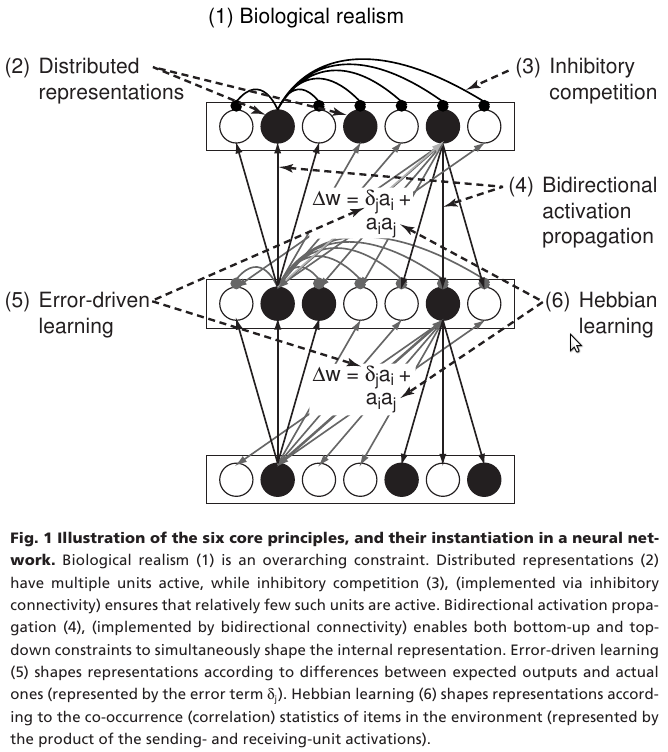
\includegraphics[width=12cm]{img/bio_plausability_o1998six.png}

    
% ==================== 11. State of the Art (or Related Work or Literature Review) =========
% In this section, you should present the theoretical basis of your work and overview of the existing solutions. When discussing on the exiting solutions you should relate and qualitatively compare them with yours.
\newpage
    %11.   State of the Art (or Related Work or Literature Review)
%In this section you should present the theoretical basis of your work and overview of the existing solutions. When discussing on the exiting solutions you should relate and qualitatively compare them with yours. This chapter should contain:

% 1) The theory and concepts of your work. For example, if you work on compiler you can mention about how compiler works without getting much into detail.

% 2) Existing state of the art solution. For example, if you implement an optimization pass, you should mention about existing optimization passes that are relevant with yours. You should emphasize the commons and differences with your solution and with the existing ones.

% You may divide this chapter in sections (e.g. each for the different existing solution).

\section{Overview}
\label{sec:overview} 

\subsection{Preliminaries}
\label{sec:theory} 

% The theory and concepts of your work. For example, if you work on compiler you can mention about how compiler works without getting much into detail.

\newcommand{\argmin}{\operatornamewithlimits{arg\,min}}
\newcommand{\Bx}{{\bf x}}
\newcommand{\By}{{\bf y}}
\newcommand{\Bh}{{\bf h}}
\newcommand{\Bw}{{\bf w}}
\newcommand{\Bc}{{\bf c}}

In this section we will describe the basics of artificial neural networks. We will also introduce the notation used in this work. Note that the definitions and notations vary through the literature. We use the one which the author is familiar with. For the reader who is comfortable with this topic we recommend to skip this section and go to related models \ref{sec:overview-models}. 

TODO notation about datasets as input / output vector, sample, sample set, training, test + citation. Stopping criterion. 

%=============================================================
\subsubsection{Perceptron.}
\label{sec:models-perceptron}

The theory behind artificial neural networks started with the model of \emph{Perceptron} introduced by~\citet{mcculloch1943logical}. It is a simple model which transforms a vector of inputs $s$ to an output value $y$. The notation as depicted on figure~\ref{fig:perceptron}: $x$ is the \emph{input vector} where always $x_0=1$, $w_{0k}$ is the \emph{weight} vector, $\Sigma$ is the \emph{summing} junction, $\eta_k$ is the \emph{net input}, $\phi$ is the \emph{activation function}, $\theta_k$ is the \emph{treshold}, $y_k$ is the \emph{output} and $b_k$ is the \emph{bias}.

\begin{figure}[H]
  \centering
  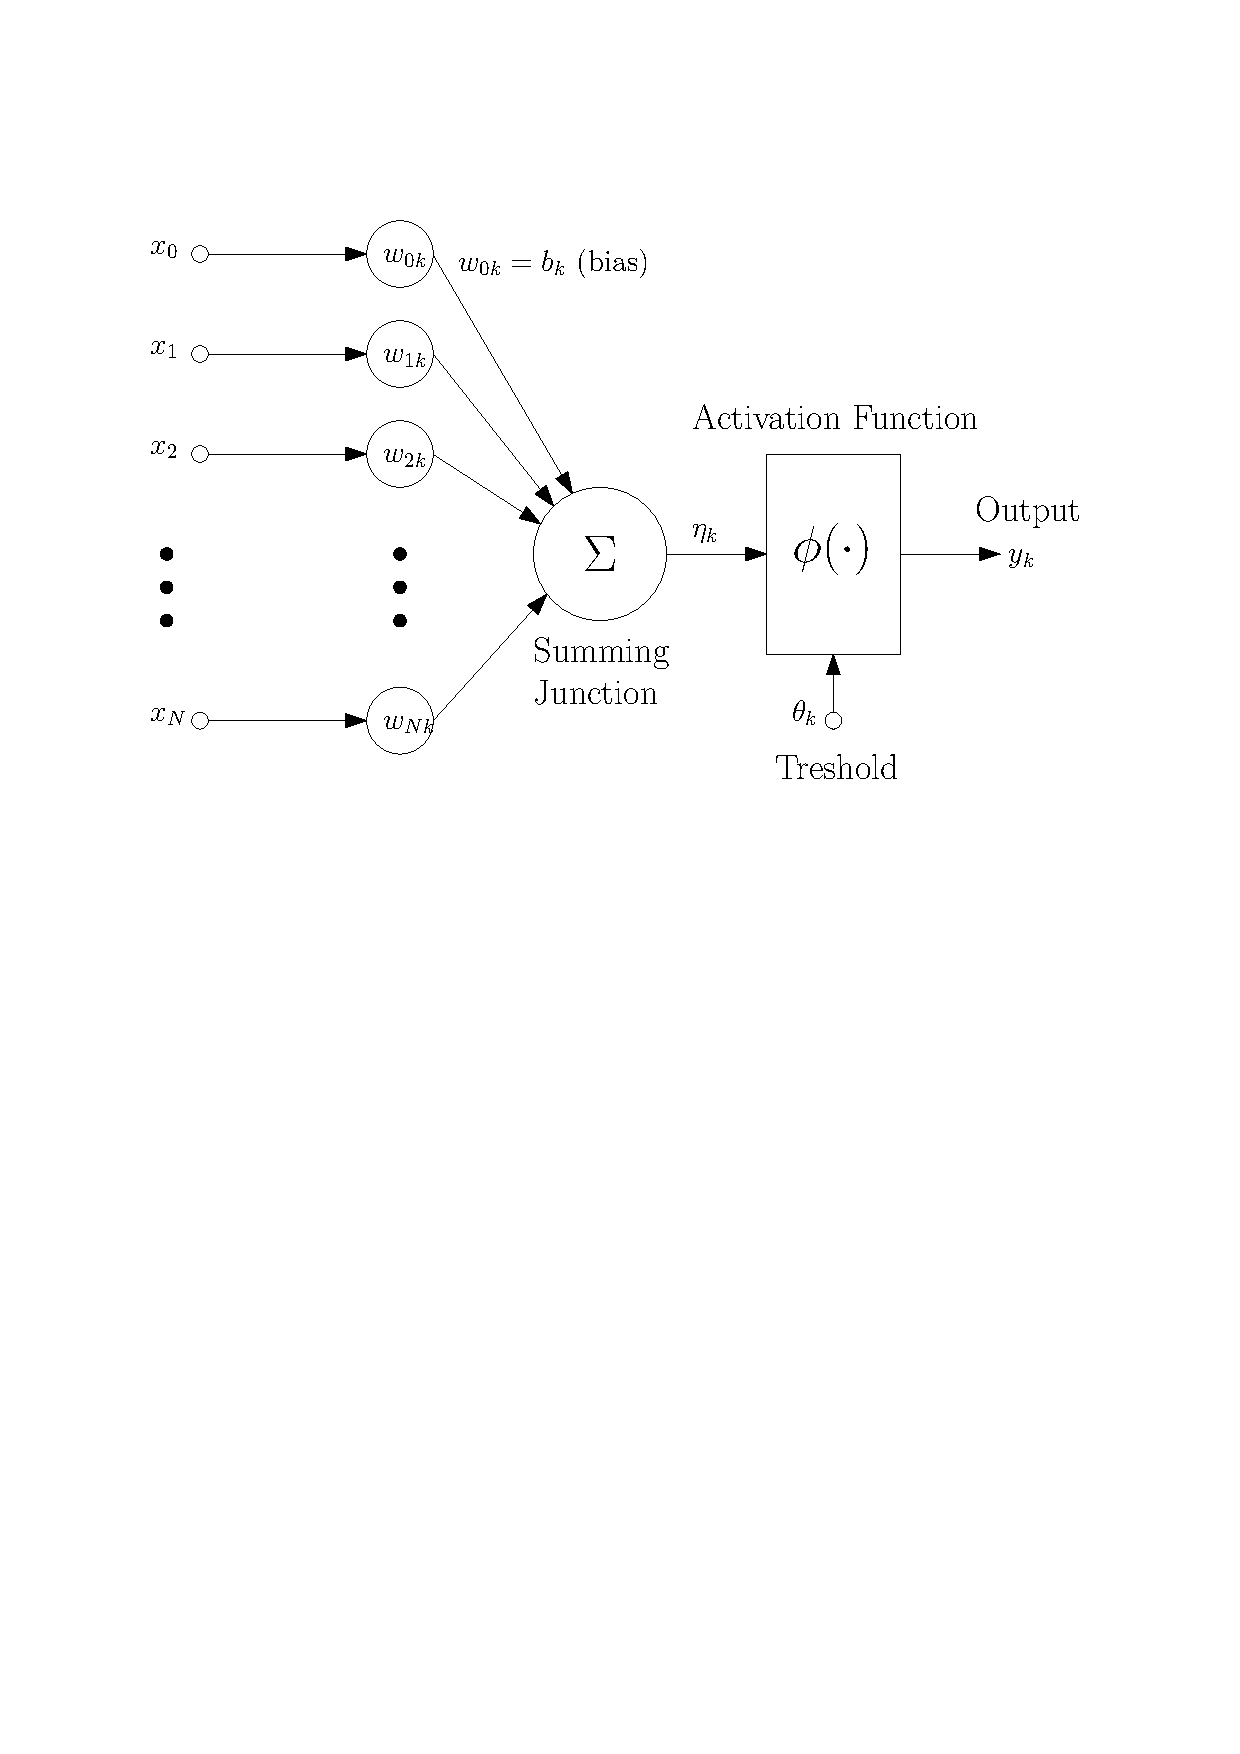
\includegraphics[width=0.6\textwidth]{img/perceptron.pdf}    
  \caption{Perceptron transforming \emph{inputs} $[x_0,\, x_1,\, \ldots,\, x_N]$ to \emph{output} $y_k$.} 
  \label{fig:perceptron}
\end{figure}

The whole transformation of the input vector to the output activation could be written as follows: 
\begin{equation}
\label{eq:perceptron} 
y_k =
\left\{
	\begin{array}{ll}
		1 & \mbox{if } \phi(\sum_{i=0}^N x_iw_{ik}) > \theta_k \\
		0 & \mbox{otherwise}
	\end{array}
\right.
\end{equation} 

Equation~\ref{eq:perceptron} describes a simple \emph{binary treshold perceptron}. One could observe that the binary perceptron divides the vector space $\mathbb{R}^N$ by a $(n-1)$--dimensional hyperplane. This behaviour was studied by~\citet{rosenblatt1958perceptron}. Now we see the importance of bias which is the absolute term in the equation of the hyperplane. \label{sec:linear-sep} This leads to the fact that for one perceptron is impossible to classify non--\emph{linearly separable} vectors. 

\paragraph{Continuous perceptron.}
We put additional constraints for the activation function $\phi : \mathbb{R} \mapsto (0,1)$ that $\phi$ is differentiable, monotonously increasing and satisfying two asymptotic conditions $t(-\infty)=0$ and $t(\infty)=1$.  Usually, the activation function is realized by the logistic function $\frac{1}{1 + \exp{-\eta}}$. To allow real numbered results from the range $(0,1)$, we drop the treshold function and simply output $\phi(\eta_k)$. 

\paragraph{Learning.} 
The goal of a perceptron is to \emph{learn} the mapping given by the set $T = \{(X^j, t_j)\}$ of pairs, where $X^j$ is the input vector $(x_{j0},x_{j1}, \ldots, x_{jN})$ and $t_j$ is the corresponding target. It could be formalized as minimizing the error function: 

\begin{equation}
\label{eq:perceptron-error} 
E = \sum_{k=1}^{N} \frac{1}{2}(t_k-y_k)^2.
\end{equation} 

A straightforward method for the network to minimize the error function \ref{eq:perceptron-error} is simply updating weights according to the partial derivates of the error function: 

\begin{equation}
\label{eq:perceptron-learning} 
\frac{\partial E}{\partial w_{ik}} = (t_k - y_k)\phi'(\eta_k)x_i = (y_k - t_k)y_k(1 - y_k)x_i,
\end{equation} 
which gives us the \emph{update rule} written as: 
\
\begin{equation} 
\label{eq:perceptron-learning-rule} 
\Delta w_{ik} = \lambda (t_k - y_k)y_k(1 - y_k)x_i,
\end{equation} 
where $\lambda$ is the \emph{learning rate}. 

Using the learning rule~(\ref{eq:perceptron-learning-rule}) and the following \emph{training} process the perceptron is able to \emph{learn}: 
%TODO check algorithm 
\begin{algorithm}[H]
  \begin{algorithmic}
    \For{$epoch = 1$ to $Epoch_{\rm max}$} 
      \ForAll{$(X^j, t_j)$ in $T$} 
        \State $y_j \gets \phi(\sum_{i=0}^N x_iw_{ik}) > \theta_k$
        \For{$i=0$ to $N$} 
          \State $w_{ij} \gets w_{ij} + \lambda (t_k - y_k)y_k(1 - y_k)x_i$
        \EndFor
      \EndFor
    \EndFor
  \end{algorithmic}
  \caption{Perceptron learning. Applying the \emph{weight update rule}~\ref{eq:perceptron-learning-rule} in loop for each sample in $T$. One main loop is called \emph{epoch}.}  
  \label{alg:perceptron-learning}
\end{algorithm} 

 
\label{sec:perceptron} 

\subsubsection{Multilayer Feedworward Networks} 
\label{sec:theory-multilayer} 

We will define \emph{multilayer feedforward networks} as in \citet{haykin1994neural}. First, we define a \emph{layered} neural network where neurons are organised to form layers. In the simplest version we have an \emph{input layer} of source nodes and an \emph{output layer} which is formed by aforementioned perceptrons. In other words this is a \emph{feedforward} or \emph{acyclic} type of network as the \emph{activation}, i.e. outputs of the neurons are computed from the input to the output layer and never \emph{backwards}. 

Multilayer neural network has one or more \emph{hidden layers} in addition to the input and ouput layer as shown on figure~\ref{fig:multilayer}. The source nodes supply the activation pattern, i.e. input vector, which is applied to second layer neurons. The output signal of the hidden layer is used as the input for the output layer. As shown by \citet{cybenko1989approximation} the three layer network is an universal approximator continuous functions on compact subsets of $\mathbb{R}^n$.

\begin{figure}[H]
  \centering
  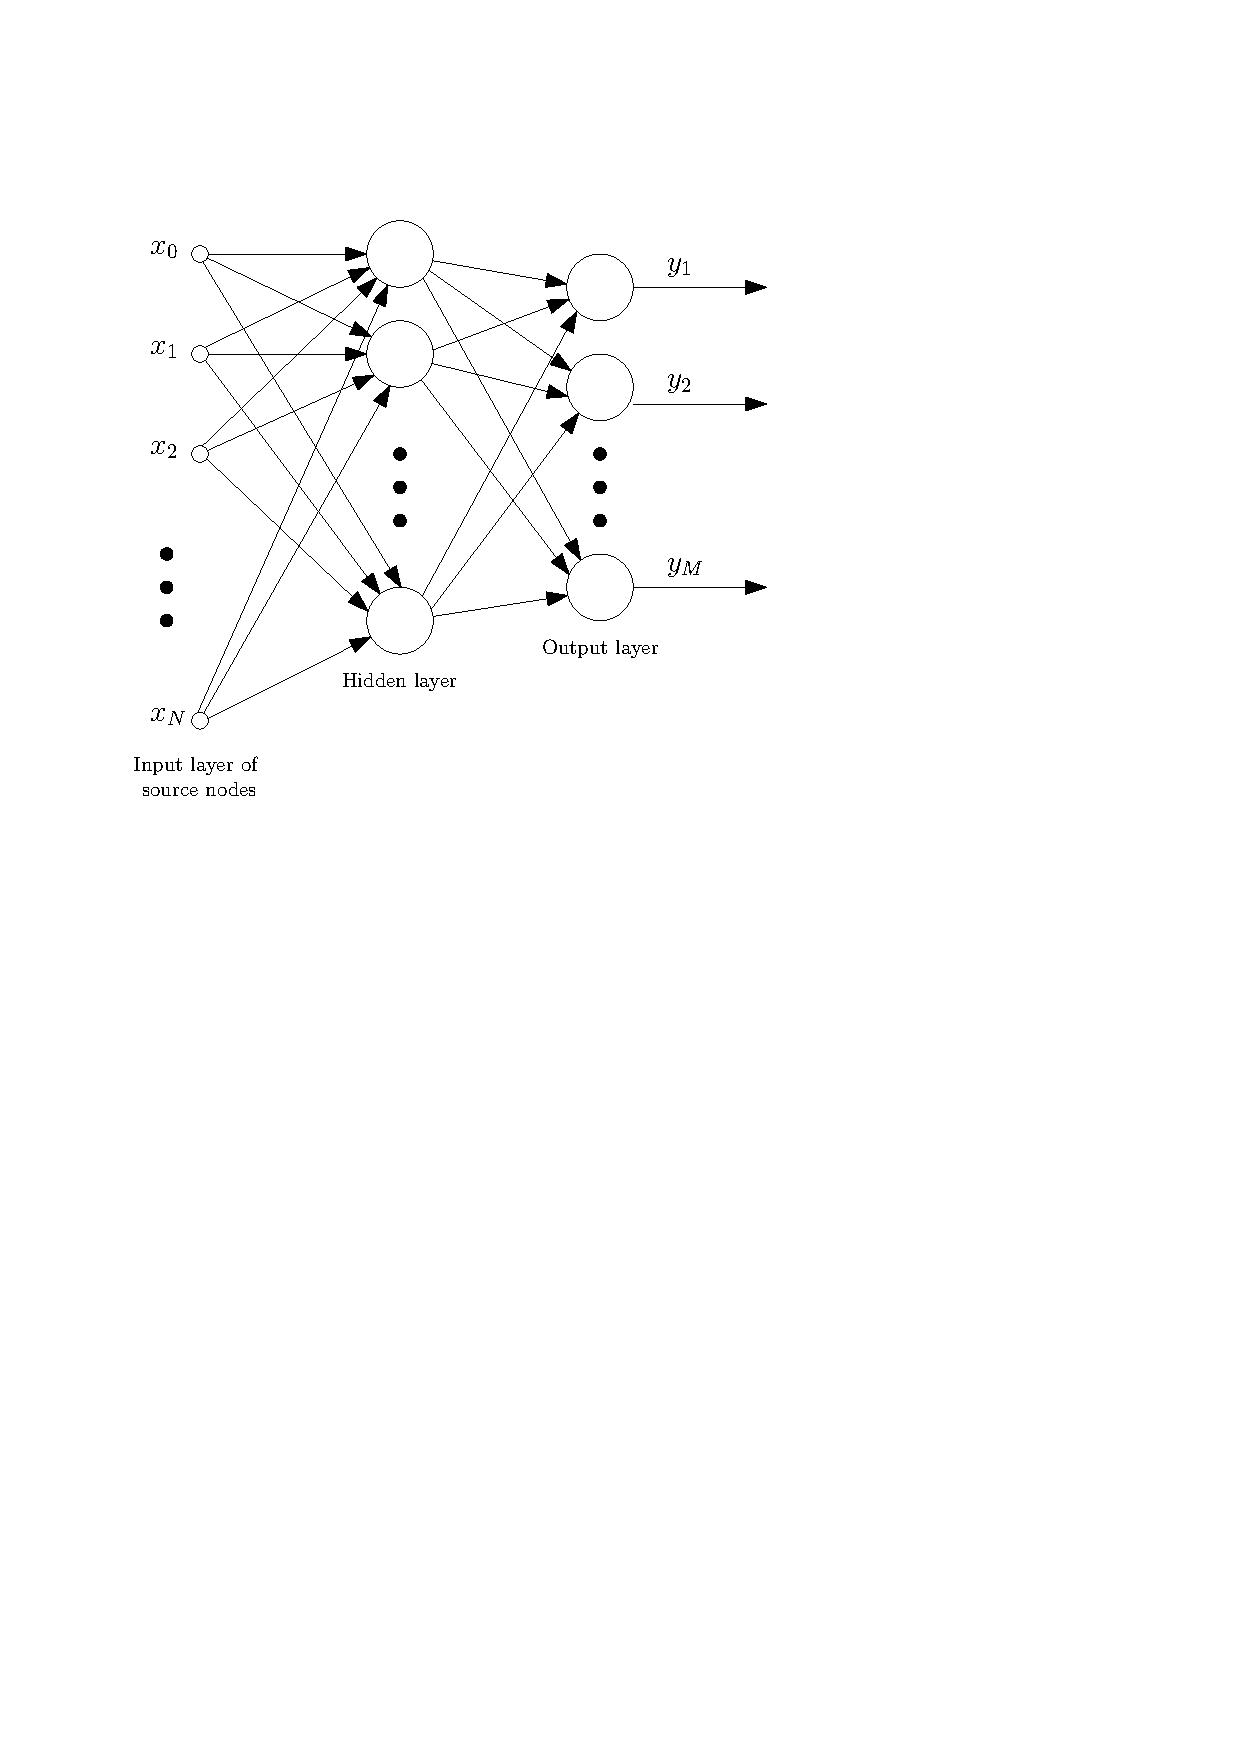
\includegraphics[width=0.5\textwidth]{img/multilayer.pdf}    
  \caption{Fully connected feedforward \emph{multilayer} network with one \emph{hidden} layer and one \emph{output} layer. } 
  \label{fig:multilayer}
\end{figure}

There exists several methods for training multilayer networks. First, we will describe the most common Backpropagation in (\ref{sec:models-bp}) and then methods related to our work such as CHL (\ref{sec:models-chl}), GeneRec (\ref{sec:models-generec}) and BAL (\ref{sec:models-bal}). 


\subsubsection{Recurrent Networks}
\label{sec:theory-recurrent} 

Recurrent networks arise problems with computing their activations. For example imagine a cycle of neurons. That means that output of a particular unit could affect its input. Therefore the activations in general couldn't be computed only by one forward pass. This introduces real--valued dynamic systems for computing the activations. We can observe that it holds that $\frac{\partial\eta}{\partial t} = 0$ for the activations of neurons in the fixed point state. There are several approaches solving these dynamic systems and deriving the learning rule \cite{pineda1987generalization, pearlmutter1989learning, williams1989learning, elman1990finding, haykin1994neural}. 

\begin{figure}[H]
  \centering
  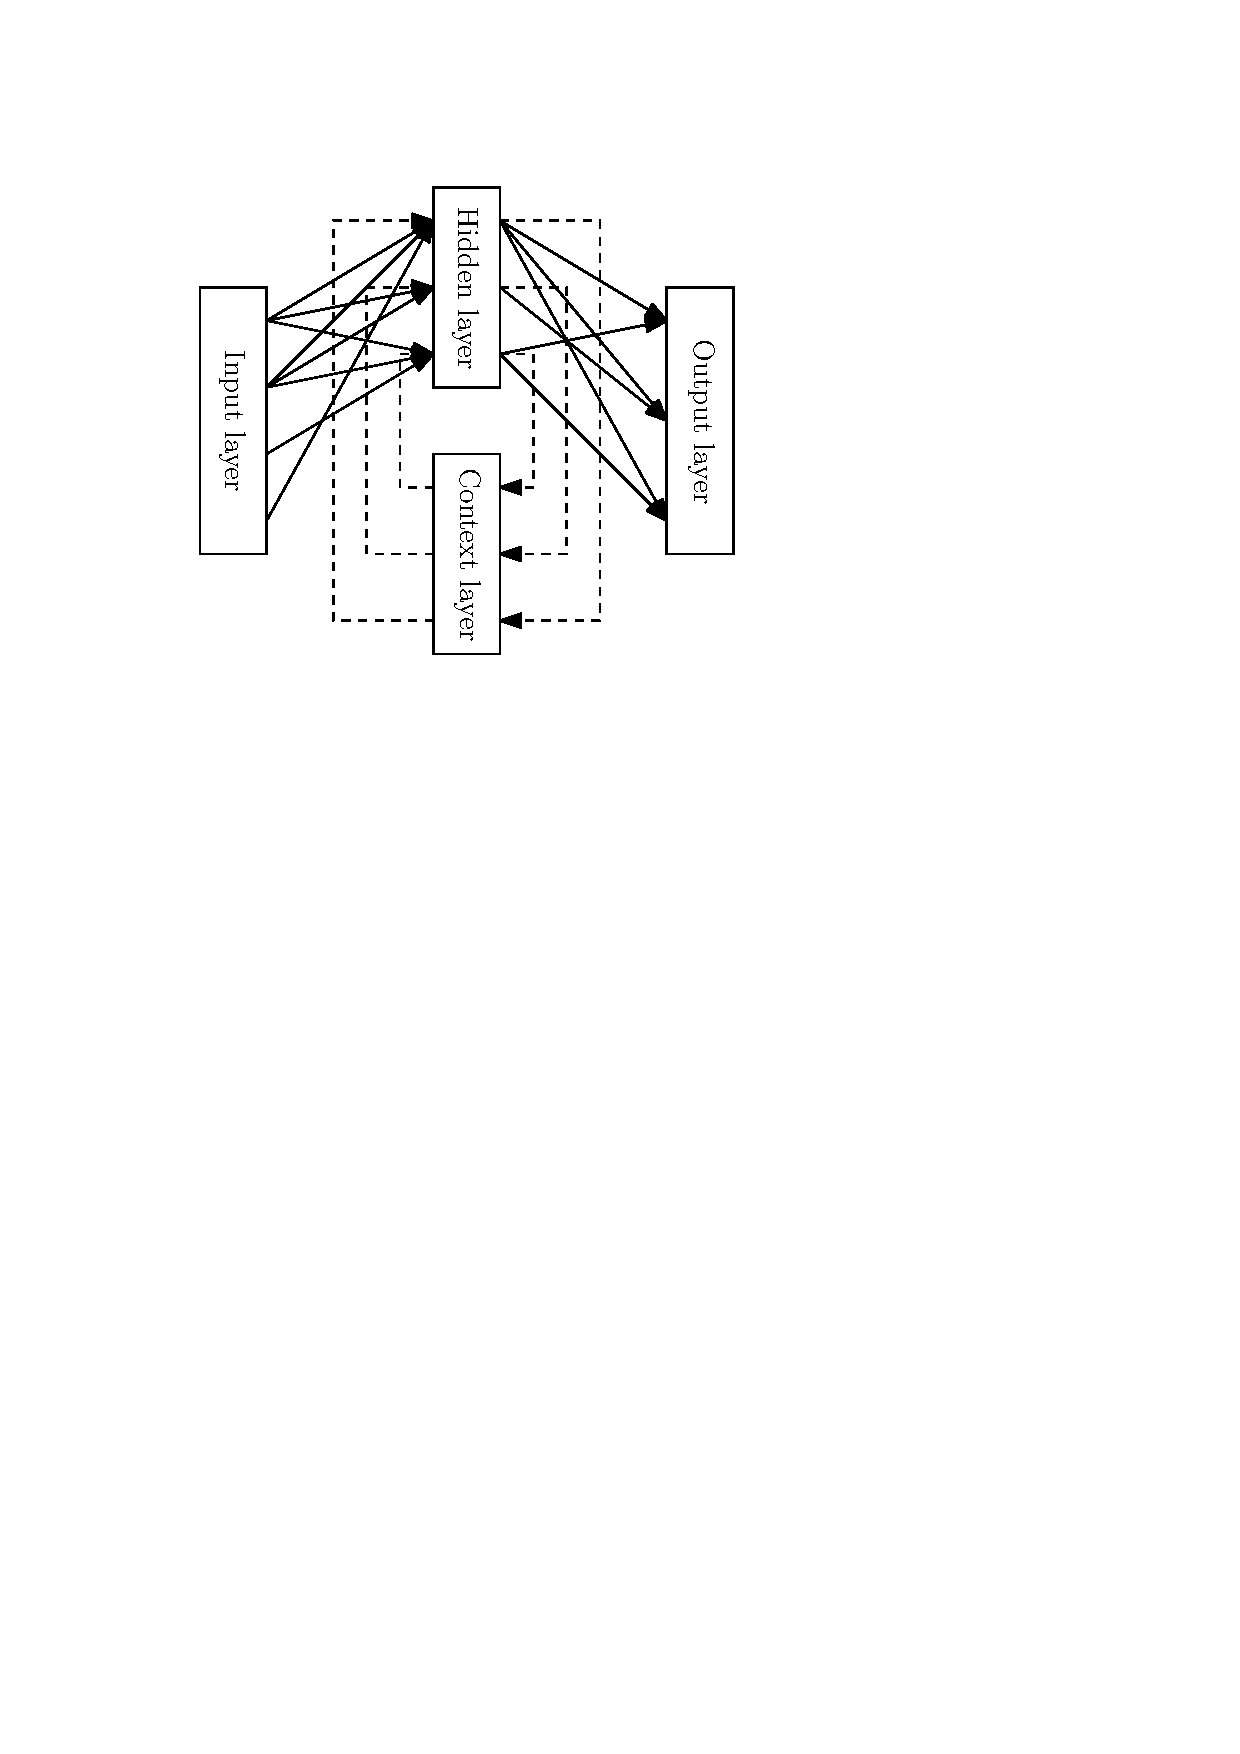
\includegraphics[width=0.4\textwidth]{img/models-recurrent.pdf}    
  \caption{Simple Recurrent network designed by \citet{elman1990finding}. Image inspiration from \citet{haykin1994neural}.} 
  \label{fig:theory-recurrent}
\end{figure}

An \emph{iterative method} is used by \citet{movellan1990contrastive} for computing activations. In the first step the input neurons have activations equal to the input vector and the other neurons have zero activation. In the next steps activations from the last step are used to compute activation in this step as shown in equation~\ref{eq:theory-recurrent-activation}: 
\begin{equation}
  \label{eq:theory-recurrent-activation} 
  \eta_i(t+1) = \phi(\sum_j w_{ji}\eta_i(t)
\end{equation}
This rule is iterated while the activation are settled. For particullar symmetric network it could be proved that activations will converge \citep{o1996bio}. For more general networks a dynamic system based on rule~\ref{eq:theory-recurrent-activation} could be derived and a fixed point solution could be found by solving a set of non--linear equations (TODO ref). \citet{movellan1990contrastive} proposes using the method of simulated annealing \citep{kirkpatrick1983optimization,vcerny1985thermodynamical} to improve the learning rule and to avoid settling the network in a local minima. We experimented with the iterative method for a two--way GeneRec \ref{sec:our-bal-recirc}. 

 

\subsubsection{Hopfield Networks}
\label{sec:theory-hopfield}

A \emph{Hopfield network} \citep{hopfield1984neurons} is a network with arbitrary connections defined only by one weight matrix $W$. Some of the units are chosen as the \emph{input units} which have stable activations for a given input pattern. We can treat a Hopfield network as a Recurrent neural network. A Hopfield network comes with an continuous error function for which usually the following function is chosen: 
\begin{equation}
  \label{eq:theory-hopfield-error}
  E = -\frac{1}{2}\sum_i\sum_ja_iw_{ij}a_j
\end{equation} 
where $a_i$ is the activation of the $i$-th unit. The aim of the network is to settle the activations so that $E$ settles in a global minimum. Activation for the $i$-th unit is computed based on the following differential equation \citep{hopfield1984neurons}: 
\begin{equation}
  \label{eq:theory-hopfield-activation}
  \frac{\partial a_i}{\partial t} = \alpha(-a_i + \phi(\eta_i)).
\end{equation} 
where $a^T = [a_1,\ldots,a_n]$ is the activation vector, $f_i$ is bounded, monotically increasing, differentiable activation function.

It could be proven for equation~\ref{eq:theory-hopfield-activation} that if the weights are symmetric, i.e. $w_{ij} = w_{ji}$, the activations will settle in the minimal error state defined by~\ref{fig:theory-hopfield-activation} \citep{hopfield1984neurons}. This learning rule is typically used in \emph{interactive activation networks} studied by \citet{grossberg1978theory, mcclelland1981interactive}. 

 
 

\subsubsection{Backpropagation}
\label{models-bp} 

TODO spomenut hetero-asociativne, jednosmerne, supervised 
TODO napisat ako theory example

A criticism of backpropagation is that it is neurally implausible (and hard to implement in hardware) because it requires all the connections to be used backward and it requires the units to use different input-output functions for the forward and backward passes \citet{hinton1988learning}.

The procedure repeatedly adjusts the weights of the connections in the network so as to minimize a measure of the difference between the actual output vector of the net and desired output vector \citet{rumelhart1986learning}. 

The aim is to find a powerful synaptic modification rule that will allow an arbitrarily connected neural network to develop an internal structure that is appropriate for a particular task domain \citet{rumelhart1986learning}. 

Connection within a layer or from higher to lower layers are forbidden, but connections can skip intermediate layers \citet{rumelhart1986learning}.

All units within a layer have their states set in parallel, but different layers have their states set sequentially, starting at the bottom and working upwards until the states of the output units are determined \citet{rumelhart1986learning}. 

$$x_j = \sum_i y_iw_{ji}.$$

$$y_i = \frac{1}{1 + e^{-x_i}}.$$

$$E = \frac{1}{2} \sum_c \sum_j (y_{j,c} - d_{j,c})^2,$$
where $c$ is index over cases. 

To minimize $E$ by gradient descent it is necessary to compute the partial derivate of $E$ with respect to each weight in the network \citet{rumelhart1986learning}. 

$$\partial E / \partial y_j = y_j - d_j.$$

We computed $\partial E / \partial y_j$ for any unit when $\partial E / \partial y_j$ given in the last layer. Repeating this procedure we get $\partial E / \partial y_j$ for all weights. 

Adding momentum:
$\Delta w(t) = -\epsilon \partial E/ \partial w(t) + \alpha \Delta w(t-1).$

Adding a few more connection creates extra dimensions in weight-space and these dimensions provide paths around the barriers that create poor local minima in the lower dimensional subspaces \citet{rumelhart1986learning}. 

The learning procedure, in its current form, is not a plausible model of learning in brains. 

$$\frac{\partial E}{\partial w_{ij}} = -\sum_k(t_k-o_k)w_{jk}\sigma'(\eta_j)s_i,$$
where $t_k$ is the target value, $o_k$ is the output value, $\sigma$ is the nonlinear function, $\eta_j$ is the net input and $s_i$ is the stimulus input \citet{o1996bio}.

%TODO prekreslit do IPE 
\begin{center} 
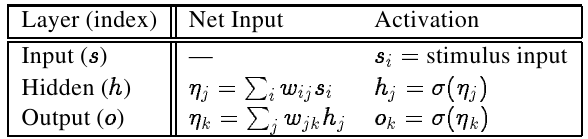
\includegraphics{img/table_bp.png} 
\citet{farkas2013bal} 
\end{center} 


\subsection{Related models} %TODO change name 
\label{sec:overview-models}  
%TODO more search - I could miss a lot (see articles which reference O'Reilly 96 ..) 
%TODO more references
%TODO made up a template for each model, like 1. motivation 2. activation table 3. learning rule
%TODO write it as a comparison to BAL-like models we analysed 

In this section we briefly mention models on which our work was based on. Mainly it's the Bidirectional Activation-based Learning algorithm \ref{sec:models-bal} by \citet{farkas2013bal} and the Generalized recirculation \ref{sec:models-generec} by \citet{o1996bio}. The other two models are inspiration for the two former ones. Understanding the latter helps understanding the former. 

%\subsubsection{Boltzmann machines}
TODO \cite{ackley1985learning}


To assess the effect of interactivity, two different networks were compared on the combinatorial generaliza-
tion task, a standard feedforward backpropagation network, and an interactive GeneRec network using the
symmetric, midpoint variation learning rule which is equivalent to contrastive Hebbian learning (CHL) or a
deterministic Boltzmann machine (DBM) \cite{o1996bio}, \cite{o2001generalization}. 

TODO: Read and cite from Hinton's original article. 

(Wiki) A Boltzmann machine is a type of stochastic recurrent neural network invented by Geoffrey Hinton and Terry Sejnowski. Boltzmann machines can be seen as the stochastic, generative counterpart of Hopfield nets. They were one of the first examples of a neural network capable of learning internal representations, and are able to represent and (given sufficient time) solve difficult combinatoric problems. If the connectivity is constrained, the learning can be made efficient enough to be useful for practical problems.

A Boltzmann machine, like a Hopfield network, is a network of units with an "energy" defined for the network. It also has binary units, but unlike Hopfield nets, Boltzmann machine units are stochastic. The global energy, $E$, in a Boltzmann machine is identical in form to that of a Hopfield network:

$$E = -\sum_{i<j} w_{ij} \, s_i \, s_j - \sum_i \theta_i \, s_i.$$

Where:
\begin{itemize}
    \item $w_{ij}$ is the connection strength between unit $j$ and unit $i$.
    \item $s_i$ is the state, $s_i \in \{0,1\}$, of unit $i$
    \item $\theta_i$ is the threshold of unit $i$.
\end{itemize}

The connections in a Boltzmann machine have two restrictions:
\begin{itemize}
    \item $w_{ii}=0\qquad \forall i$. (No unit has a connection with itself.)
    \item $w_{ij}=w_{ji}\qquad \forall i,j$. (All connections are symmetric.)
\end{itemize}

Often the weights are represented in matrix form with a symmetric matrix $W$, with zeros along the diagonal.

\paragraph{Hopfield nets.}

TODO: Read and cite from Hopfields's original article. (Storkey, Amos. "Increasing the capacity of a Hopfield network without sacrificing functionality." Artificial Neural Networks—ICANN'97 (1997): 451-456.)

(Wiki) A Hopfield network is a form of recurrent artificial neural network invented by John Hopfield. Hopfield nets serve as content-addressable memory systems with binary threshold nodes. They are guaranteed to converge to a local minimum, but convergence to a false pattern (wrong local minimum) rather than the stored pattern (expected local minimum) can occur. Hopfield networks also provide a model for understanding human memory.

\paragraph{Boltzmann distribution.}

TODO:  Landau, Lev Davidovich; and Lifshitz, Evgeny Mikhailovich (1980) [1976]. Statistical Physics. 5 (3 ed.). Oxford: Pergamon Press. ISBN 0-7506-3372-7. Translated by J.B. Sykes and M.J. Kearsley. See section 28

(Wiki) The Boltzmann distribution for the fractional number of particles $Ni / N$ occupying a set of states $i$ possessing energy $E_i$ is:

    $${N_i \over N} = {g_i e^{-E_i/(k_BT)} \over Z(T)}.$$

where $k_B$ is the Boltzmann constant, $T$ is temperature (assumed to be a well-defined quantity), $g_i$ is the degeneracy (meaning, the number of levels having energy $E_i$; sometimes, the more general \'states\' are used instead of levels, to avoid using degeneracy in the equation), $N$ is the total number of particles and $Z(T)$ is the partition function.

    $$N=\sum_i N_i,$$

    $$Z(T)=\sum_i g_i e^{-E_i/(k_BT)}. $$
  %moved to old 

%\def\myover#1#2{\mathrel{\overset{\makebox[0pt]{#2}}{#1}}}
%\newcommand{\mytilde}{\raise.17ex\hbox{$\scriptstyle\mathtt{\sim}$}}
%\def\myequi#1{\myover{#1}{\mytilde}}

\subsubsection{Contrastive Hebbian learning}
\label{sec:models-chl} 

The main idea of \emph{Contrastive Hebbian Learning} developed by~\citet{movellan1990contrastive} is to have two activation phases in an aribtrary Hopfield network~\citep{hopfield1984neurons} as described in~Section~\ref{sec:theory-hopfield}. In the first phase, called \emph{minus phase} and denoted ``$-$'', only the input vector is \emph{clamped}, i.e. activations of the clamped units as equal to the clamped values. In the second phase, called \emph{plus phase} and denoted ``$+$'', both the input and target are clambed to the underlying network. The learning is based on the difference of these two activations. For an idea how it works see Table~\ref{tab:models-generec}. Note that CHL makes no assumptions about the structure of the underlying network and therefore, it has no layers in general. 

\newpage
As mentioned previously CHL is based on Hopfield networks. Therefore, it has an energy function $J$ which is based on the Helmholtz free energy function $F$~\citep{hinton1989deterministic}:
\begin{equation}
  \label{eq:models-chl-helmholtz}
  F = -\frac{1}{2}\sum_i\sum_ja_iw_{ij}a_j + \sum_i \int_{f(0)}^{a_i} f_i^{-1}(a)da
\end{equation} 
where $-\frac{1}{2}\sum_i\sum_ja_iw_{ij}a_j$ is the Hopfield energy function~(\ref{eq:theory-hopfield-energy}). Then the \emph{contrastive} error function $J$ is defined as: 
\begin{equation}
  \label{eq:models-chl-energy}
  J = \hat{F^{+}} - \hat{F^{-}}
\end{equation} 
where $\hat{F^{+}}$ and $\hat{F^{-}}$ respectively are the values of the energy functions at equilibrium states for the plus and the minus phases. 

Based on the contrastive energy function~(\ref{eq:models-chl-energy}) a~learning rule is derived by~\citet{movellan1990contrastive}: 
\begin{equation}
  \label{eq:models-chl-learning-rule}
  \Delta w_{ij} = \hat{a_i}^{+}\hat{a_j}^{+} - \hat{a_i}^{-}\hat{a_j}^{-}
\end{equation}
where $\hat{a_i}$ and $\hat{a_j}$ denote the equilibrium state activations of the $i$--th and $j$--th unit. It could be shown that the learning rule~(\ref{eq:models-chl-learning-rule}) decreases the energy function~(\ref{eq:models-chl-energy})~\citep{movellan1990contrastive}. Moreover it could be shown that the CHL learning rule is equivalent to backpropagation learning rule in terms of computability while it is biologically more plausible as it uses only activation for computing the error gradient~\citep{o1996bio, xie2003equivalence}. 

   


%\subsubsection{Almeida-Pineda Algorithm}

Pineda first applied the backpropagation rule to recurrent networks. Recurrent networks can have cycles and they contain no layers. Subset $\Omega$ of the units is treated as the output layer. So the Almeida-Pineda network is a generealization of the backpropagation network. 

As the network is recurrent it can remember information and can be used as CAM.
%TODO citation for CAM 

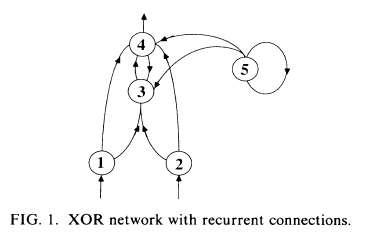
\includegraphics[width=8px]{img/recurrent.png}

\paragraph{My notes.} 
So the Pinedas NS is a dynamical system which should converge and converges for forward/backward nets (quite trivially). 

The delta rule is constructed to move the state towards the fixed point which is defined so that the difference on output neurons is equal to zero (values on other neurons are chosen arbitrary?). 

First Pineda derives an exact learning rule which requires computation of inverse matrix what is both bad for implementation and biological plausibility. So it is simplified to associate dynamical system (I don't understand how) which converges if the original dynamical system converges (proved by Almeida). 

It is more natural as all neurons are equivalent by construction. The advantage is exploited in hardware computation as it treats differential equations more naturally can be solved by analog computers. 

%TODO: Compare this conclusion with O'Reillys. 


TODO: Understand the basics of differential equations to enhance the intuition about learning rules. 

TODO: Study the Lapedes and Farber: master / slave NS. 

\paragraph{Citations from the article.}

Nevertheless it has been applied to recurrent networks by taking advanage of the fact that for every recurrent network there exists an equivalent feedforward network (for a finite time) \cite{pineda1987generalization}.

Hopfield's equations are globally asymptotically stable if $w$ is symmetric and has zeros along the diagonal \cite{pineda1987generalization}.

$$y_r = \beta f_r^,(u_r)\sum_k J_k(L^{-1})_{kr},$$
where 
$$L_{ij} = \alpha \delta_{ij} - \beta f_i^,(u_i)w_{ij},$$
and where $\delta_{ij}$ is the Kronecker $\delta$ symbol and $J_i = t_t - x_i$ if $i \in \Omega$ and $J_i = 0$ otherwise \cite{pineda1987generalization}. 

Then the exact learning rule is 
$$dw_{rs}/dt = \gamma y_r x_s.$$
Rhis exact learning rule needs matrix inversion to calculate the error signals $y_k$. Direct matrix inversions are necessarily nonlocal calculations and therefore this learning algorithm is not suitable for implementation as a neural network \cite{pineda1987generalization}. 

TODO: Understand the associated dynamical system and the new learning rule (page 3/4). 

\paragraph{O'Reillys conclusion}
\cite{o1996bio}
The activation states in AP are updated according to a discrete-time approximation of the following dif-
ferential equation, which is integrated over time with respect to the net input terms :

$$\frac{d\eta_j}{d_t} = -\eta_j + \sum w_{ij} \sigma(\eta_i).$$

This equation can be iteratively applied until the network settles into a stable equilibrium state (i.e., until the
change in activation state goes below a small threshold value), which it will provably do if the weights are
symmetric (Hopfield, 1984), and often even if they are not (Galland \& Hinton, 1991).

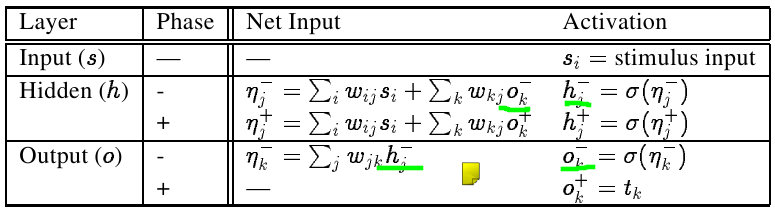
\includegraphics[width=10cm]{img/table_ap.png}
  %moved to old 

\subsubsection{Recirculation algorithm}
\label{sec:models-recirc} 

The \emph{Recirculation algorithm} designed by \citet{hinton1988learning} is an unsupervised neural letwork for learning encoder tasks. Motivation for such a model comes from interesting hidden representations of Backpropagation (\ref{sec:models-bp}) with possible usage as an encoder. It has only two layers denoted \emph{visible layer} and \emph{hidden layer} as shown on figure~\ref{fig:models-recirc}. The aim of the network is to remember on the hidden layer the patterns presented to the visible layer. This could be used for compression if the hidden layer has less units than the visible layer. It also could be used as a content--accessed--memory where if novel patterns are presented to the network it could show the most similar stored pattern. 

\begin{figure}[H]
  \centering
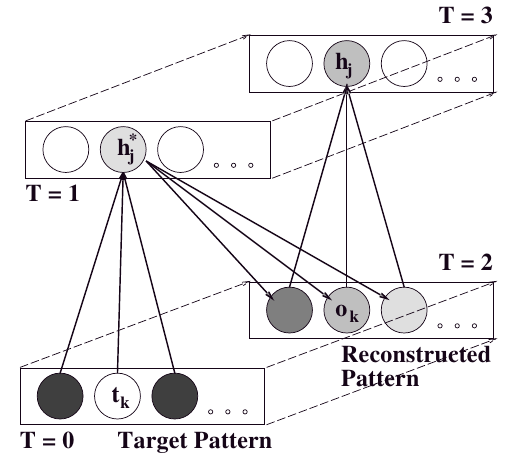
\includegraphics[width=0.4\textwidth]{img/recirculation.png}
  \caption{The recirculation algorithm by \citet{hinton1988learning}. }
  \label{fig:models-recirc}
\end{figure}

As depicted on \ref{fig:models-recirc} activation is propagated in four steps $T \in \{0,1,2,3\}$. At the first phase denoted by $T=0$ only the input vector $t$ is clamped on the visible layer, at $T=1$ a forward pass $h^{*}$ is computed from visible to hidden, at $T=2$ a reconstructed pattern $o_k$ as a function of hidden state $h^{*}$ at $T=1$ is computed and finally at $T=3$ a hidden state $h$ is computed from $o_k$.

For the reconstruction to work \emph{symmetric} weights are used. The learning rule is common for both visible and hidden layers and it;s based only on difference of activations: 
\begin{align}
\frac{\partial E}{\partial w_{ij}} &= -(\eta^{*}_j - \eta_j) \phi'(\eta_j) t_k \nonumber \\
&\approx -(h^{*}_j - h_j)t_k \nonumber 
\end{align} 
The approximation step could be made because $\phi'(\eta_j)$ has \emph{usually} same sign as $(\eta^{*}_j - \eta_j) $ \citep{hinton1988learning, o1996bio}. The approximation works better if the difference of activations is smaller and therefore the activation for the reconstructed pattern $o$  is made similar to target pattern $t$: 
\begin{equation}
o_k = \alpha t_k + (1-\alpha)f(\eta_k). 
\end{equation} 

%Authors study the case of asymetric weights. They do not provide a proof of convergence but they provide some intutition why it should work. Also they link the work of Ballard who experimented with connecting (merging) several closed loops so that hidden units of closed loops can be input units of other closed loops of recirculation.

%\paragraph{From the original article.}
%Instead of using a separate group of units for the input and output we use the very same group of \textit{visible} units, so the input vector is the initial state of this group and the output vector is the state after information has passed around the loop. The difference between the activity of a visible unit before and after sending activity around the loop is the derivative of the squared reconstruction error \citet{hinton1988learning}.

%On the first pass, the original visible vector is passed around the loop, and on the second pass ana average of the original vector and the reconstructed vector is passed around the loop. The learning procedure changes each weight by an amount proportional to the product of the \textit{presynaptic} activity and the \textit{difference} in the post-synaptic activity on the two passes  \citet{hinton1988learning}.



%\subsubsection{Deep architectures}
Theoretical results strongly suggest that in order to learn the kind of complicated functions that can represent high-level abstractions (e.g. in vision, language, and other AI-level tasks), one needs deep architectures. Deep architectures are composed of multiple levels of non-linear operations, such as in neural nets with many hidden layers or in complicated propositional formulae re-using many sub-formulae. Searching the parameter space of deep architectures is a difficult optimization task, but learning algorithms such as those for Deep Belief Networks have recently been proposed to tackle this problem with notable success, beating the state-of-the-art in certain areas. This paper discusses the motivations and principles regarding learning algorithms for deep architectures, in particular those exploiting as building blocks unsupervised learning of single-layer models such as Restricted Boltzmann Machines, used to construct deeper models such as Deep Belief Networks \cite{bengio2009learning} (Abstract copied).

TODO read the article. 
 %moved to old 

\subsubsection{Generalized recirculation}
\label{sec:models-generec} 

\paragraph{Introduction.} 
The \emph{Generalized recirculation algorithm}, or \emph{GeneRec}, was developed by \citet{o1996bio}. It's a supervised algorithm which in comparison with Backpropagation (\ref{sec:models-bp}) is argued to be a more biologically plausible model as error is computed locally as a difference between activations \citep{o1998six, o2001generalization, da2011advances, schneider2009application}. In summary, GeneRec is a combination of CHL (\ref{sec:models-chl}) and the Recirculation algorithm (\ref{sec:models-recirc}). It overcomes limitations of the Recirculation algorithm to be an encoder by having a three layer network. For the error computation a backward weight matrix from output layer to hidden layer is used and the learning rule is derived from the CHL learning rule~\ref{eq:models-chl-learning-rule}. It could be proven that GeneRec, as Backpropagation, could learn arbitrary input--output mappings \citep{o1996bio}. 

\paragraph{Learning rule.} 
\label{sec:models-generec-learning-rule} 
GeneRec uses three weight matrices $W^{IH}$, $W^{HO}$ and $W^{OH}$ for the input--hidden, hidden--output and output--hidden weights. It also has the \quotes{-} and \quotes{+} phases as CHL with same meaning, i.e. in the \emph{minus} phase only the input vector is clamped and in the \emph{plus} phase both input and target vectors are clamped as seen on table~\ref{tab:models-generec}. Generec uses the non--symmetric version of the CHL rule for all three weight matrices: 
\begin{equation}
  \label{eq:models-generec-learning-rule}
  \Delta w_{ij} = \lambda a^{-}_i(a^{+}_j - a^{-}_j)
\end{equation}
where $a^{-}_p$ denotes the presynaptic and $a^{-}_q$ denotes the postsynaptic unit activation in minus phase, $a^{+}_p$ is the presynaptic activation from plus phase and $\lambda$ denotes the learning rate. So for example when updating $W^{HI}$ then $a^{-}_i = h^{-}_i$, $a^{-}_j = o^{-}_j$ and $a^{+}_j = t_k$. 

\paragraph{Activation.} 
\label{sec:models-generec-activation} 
The main difference between CHL and GeneRec is that GeneRec has layers and it's based more on Recurrent neural networks than on the Hopfield networks. Therefore, as shown in table~\ref{tab:models-generec}, we can compute the activations sequentially. 
\begin{table}[H]
  \centering
  \begin{tabular}{|cccc|}
    \hline
    Layer & Phase & Net Input & Activation\\
    \hline
    Input (s)    & $-$ & - & $s_i$ = \mbox{stimulus input} \\
    \hline
    Hidden (h)   & $-$ & \hspace{0.3cm}$\eta^{-}_j = \sum_i w_{ij}^{IH}s_i + \sum_k w_{kj}^{OH}o^{-}_k$\hspace{0.3cm} &
    $h^{-}_j = \sigma(\eta^{-}_j)$\hspace{0.3cm}\\
          &  +  & $\eta^{+}_j = \sum_{i}w_{ij}^{IH}s_i + \sum_k w_{kj}^{OH}o^{+}_k$ & $h^{+}_{j} = \sigma(\eta^{+}_j)$ \\
    \hline
    Output (o) & $-$ & $\eta^{-}_k = \sum_j w_{jk}^{HO}h_j$ & $o^{-}_k = \sigma(\eta^{-}_k)$\\
           &  +  & - & $o^{+}_k$ = \mbox{target output} \\
    \hline
  \end{tabular}
  \caption{Equilibrium network variables in GeneRec model \citet{o1996bio}. We can see the inspiration from the Recirculation algorithm (\ref{sec:models-recirc}) and a correspondence between $T$ and GeneRec phases. In particular $s^{-} \approx T=0$, $h^{-} \approx T=1$, $o^{-} \approx T=2$ and $h^{+}$ corresponds to $T=3$. The activation flow is depicted on figure~\ref{fig:models-generec-phase}.}
  \label{tab:models-generec}
\end{table}
In case of the \emph{plus} phase only the hidden activations are necessary to compute what could be achieved by computing $\phi(\eta_i)$. In case of the \emph{minus} phase where only inputs are clamped it's necessary to find an \emph{equilibrium} activation state for which the equations~\ref{tab:models-generec} hold. As dicussed in recurrent networks~(\ref{sec:theory-recurrent}) there are several approaches. In our implementation~(\ref{sec:appendix-impl-generec}) we choose the \emph{iterative method} with following rules for computing activations $a_i$: 
\begin{align}
  \label{eq:models-generec-activation}
  a_i(0) &= \left\{
	\begin{array}{ll}
		s_i & \mbox{if } i \in \mbox{input} \nonumber \\
		0 & \mbox{otherwise} \nonumber 
	\end{array}
\right. \\
  a_i(t+1) &= \left\{
	\begin{array}{ll}
		s_i & \mbox{if } i \in \mbox{input} \nonumber \\
		\phi(\sum_j w_{ji}a_j(t)) & \mbox{otherwise} \nonumber 
	\end{array}
\right. \\
\end{align} 
where $a_i(t)$ is the activation of $i$--th unit in discrete time $t$. The rules~\ref{eq:models-generec-activation} while are iterated while $|a_i(t+1) a_i(t)| > \epsilon$ for some unit $i$. This method is further discussed in (\ref{sec:generec-fluctuation}) and \citep{orru2008sabio}.

\begin{figure}[H]
  \centering
  %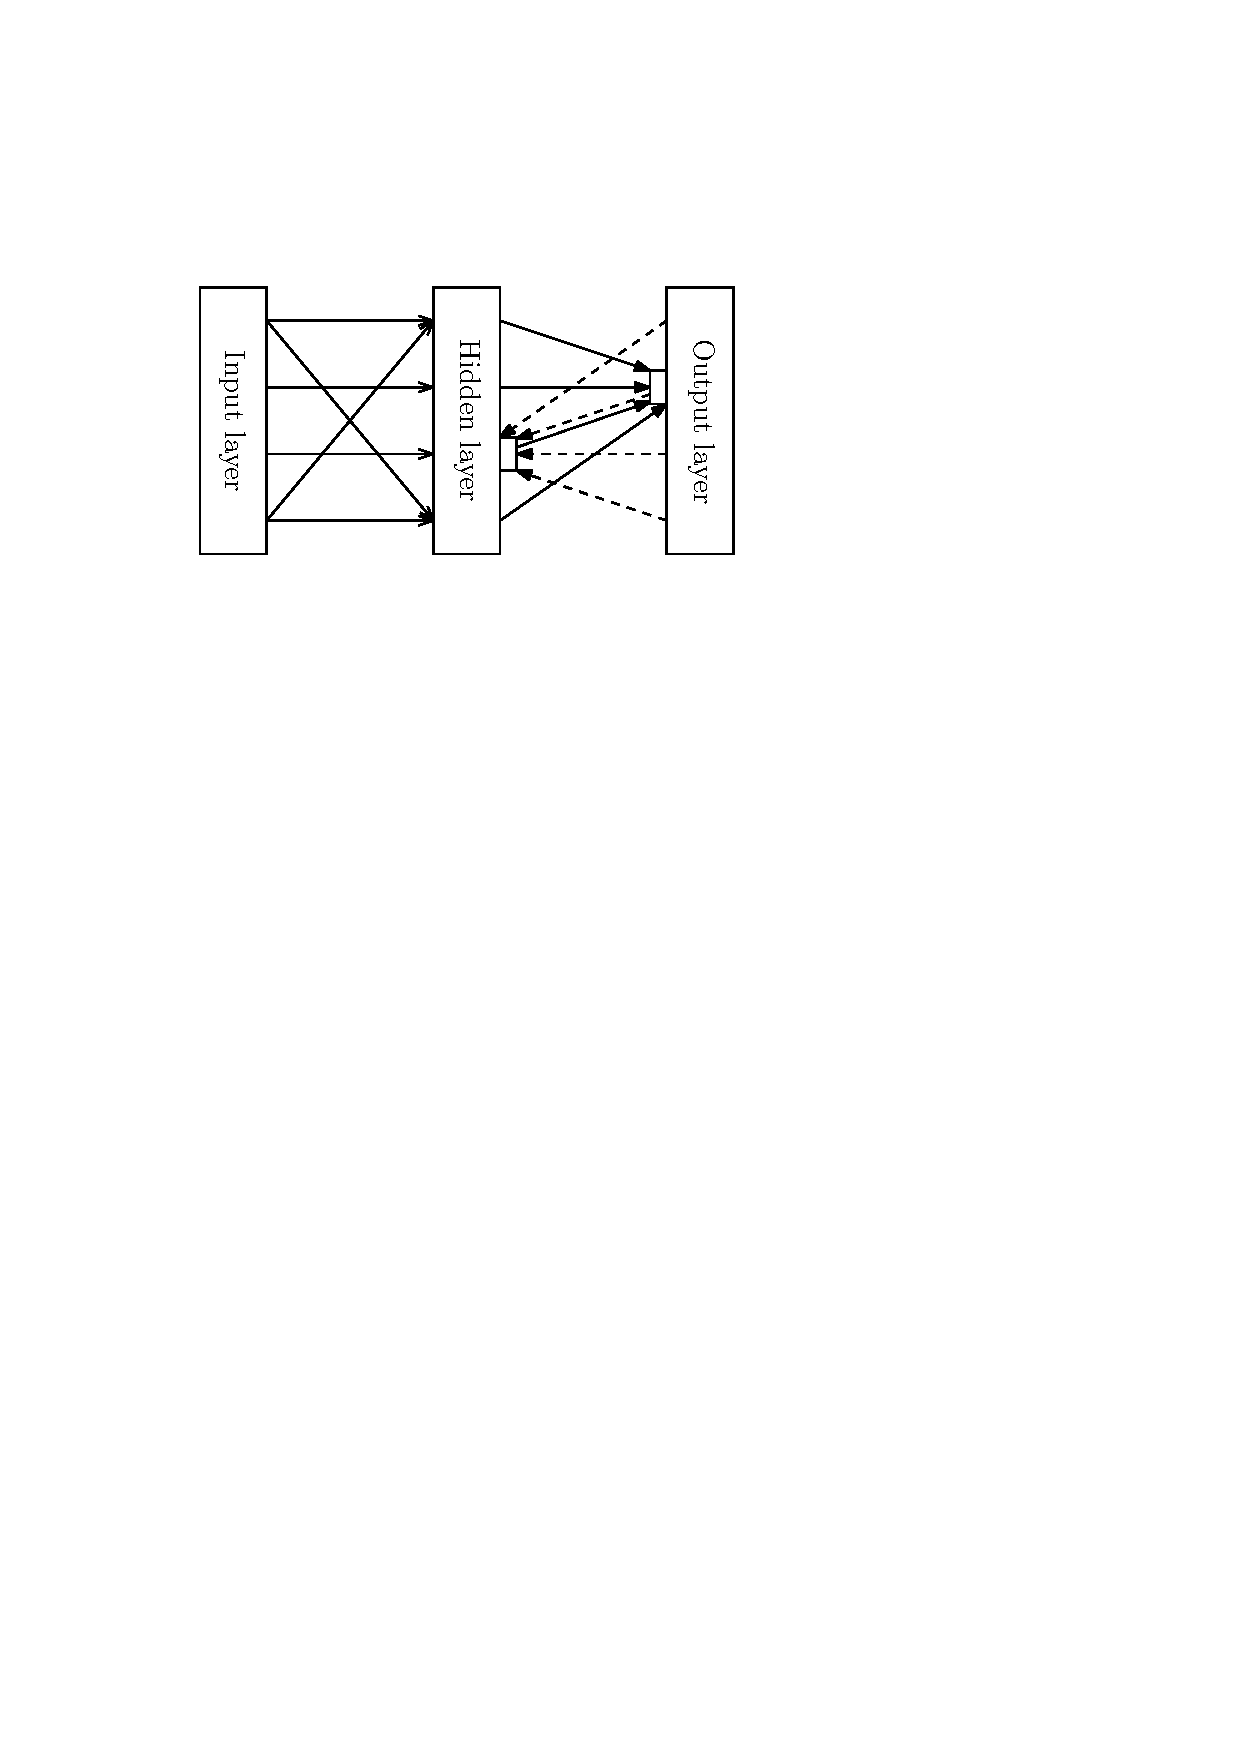
\includegraphics[width=0.4\textwidth,left]{img/models-generec-minus-phase.pdf}
  %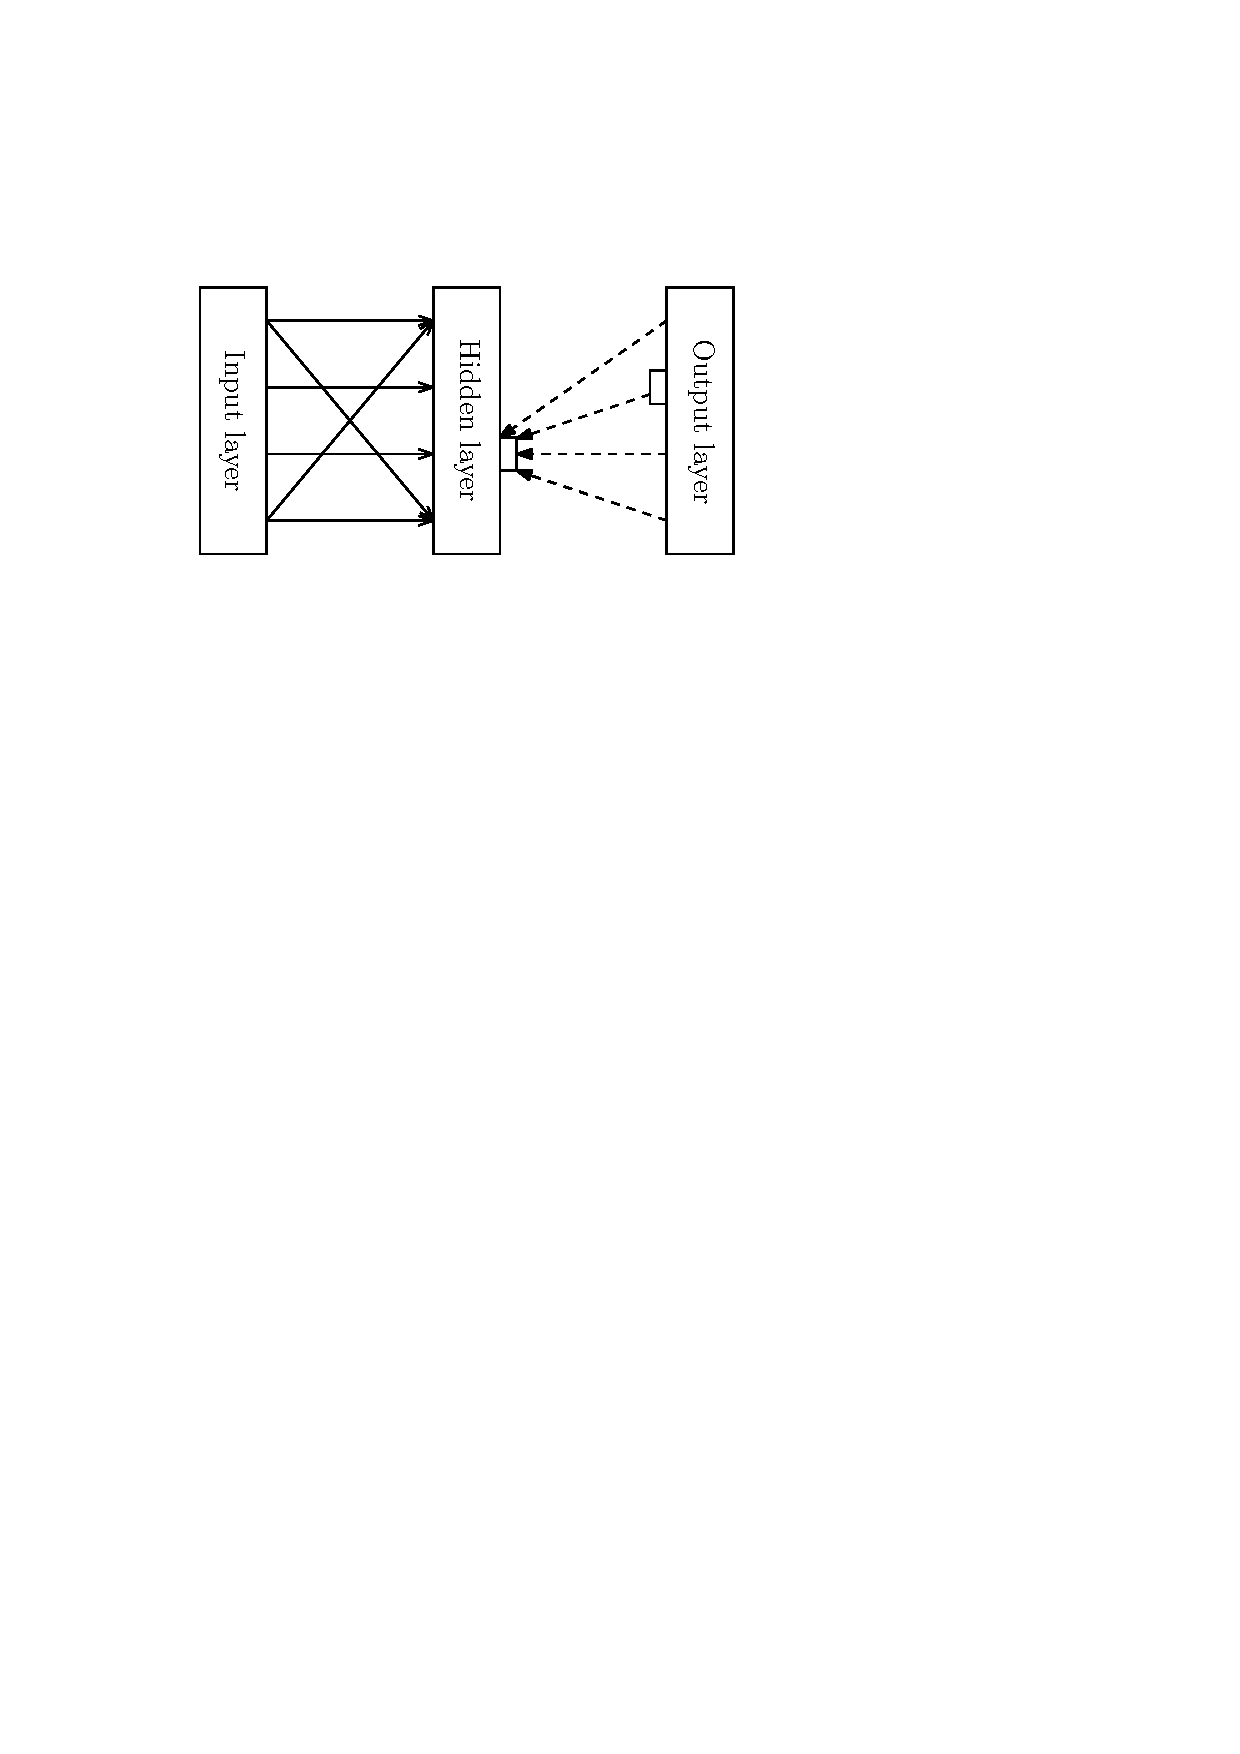
\includegraphics[width=0.4\textwidth,right]{img/models-generec-plus-phase.pdf}
  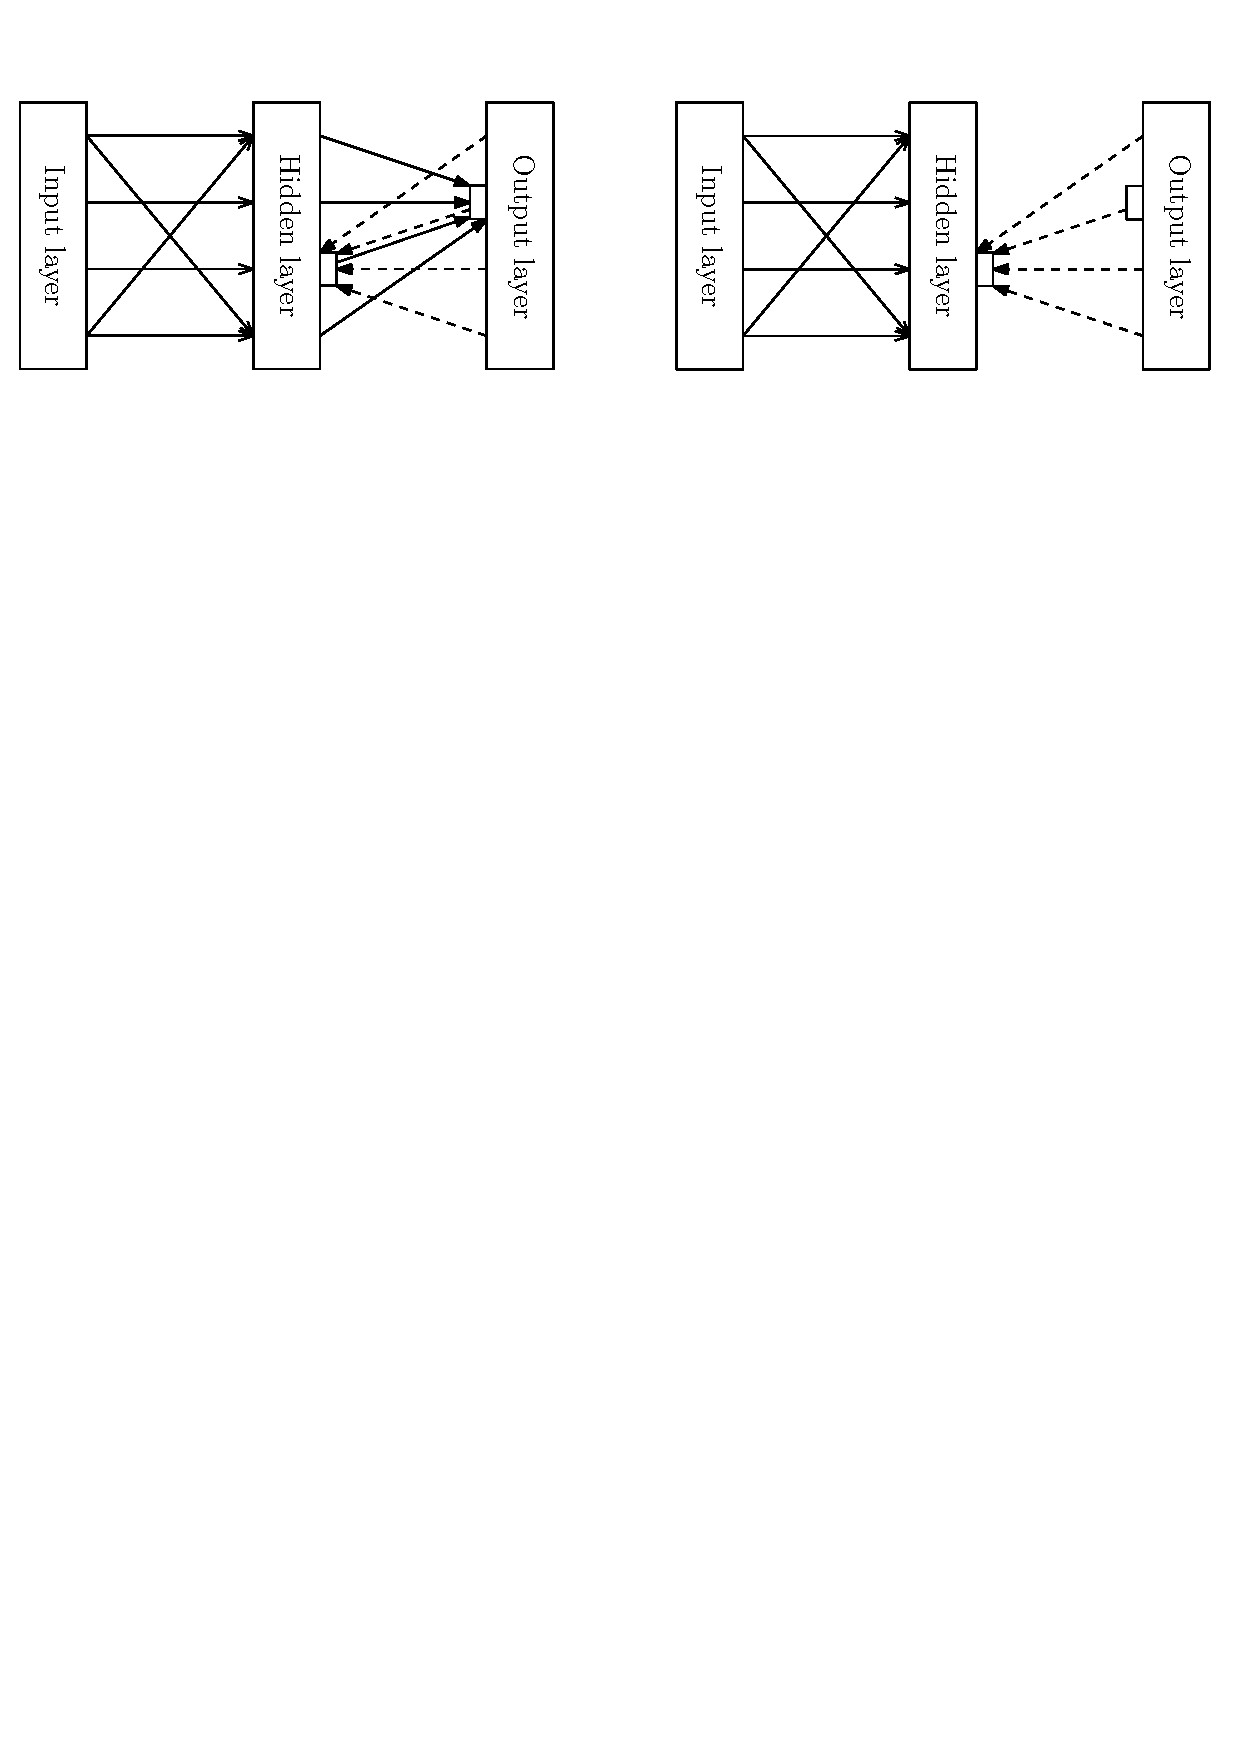
\includegraphics[width=0.8\textwidth]{img/models-generec-phase.pdf}
  
  \caption{Depicting the minus (left) and plus (right) phases of GeneRec defined in table~\ref{tab:models-generec}. Picture inspiration from \citet{orru2008sabio}.} 
  \label{fig:models-generec-phase}
\end{figure}

\paragraph{Modifications.}
\label{sec:our-learning-rules}
\label{sec:models-generec-modifications} 
It's important to note that \citet{o1996bio} proved that GeneRec converges if the learning rule~\ref{eq:models-generec-learning-rule} is a valid approximation to the error derivate and the weights beeing symmetric, i.e. $W^{HO} = W^{OH^{T}}$. \citet{o1996bio} based on CHL and the midpoint method for fradient computation \citep{press1990numerical} proposed two more learning rules for GeneRec: 
\begin{equation}
  \label{eq:models-generec-learning-rule-mid}
  \frac{1}{\lambda} \Delta w_{ij} =  \frac{1}{2}(a^{-}_i + a^{+}_i)(a^{+}_j - a^{-}_j)
\end{equation}
\begin{equation}
  \label{eq:models-generec-learning-rule-sym}
  \frac{1}{\lambda} \Delta w_{ij} =  (a^{+}_j a^{-}_i - a^{-}_j a^{+}_i) - 2a^{-}_j a^{-}_i
\end{equation}
where~\ref{eq:models-generec-learning-rule-mid} is called the \emph{midpoint learning rule} and~\ref{eq:models-generec-learning-rule-sym} is called the \emph{symmetric learning rule} which aims to preserve weight symmetry. By combining rules ref{eq:models-generec-learning-rule-mid} and \ref{eq:models-generec-learning-rule-sym} we get the following rule: 
\begin{equation}
  \label{eq:models-generec-learning-rule-chl}
  \frac{1}{\lambda} \Delta w_{ij} =  (a^{+}_i a^{+}_j) - (a^{-}_i a^{-}_j)
\end{equation}
which is indeed the CHL learning rule~\ref{eq:models-chl-learning-rule}. Thus we see that GeneRec is closely related to CHL. 

Note that we encountered some missing details in \citet{o1996bio} about how to implement the GeneRec algorithm which are further discussed in (\ref{sec:appendix-impl-generec}).


%==================== 12.   Background overview (optional) ======
\subsection{Bidirectional Activation-based Learning algorithm} 
\label{sec:models-bal} 
% If your work builds on top of an existing one, this is the place to describe the existing work in more detail, pointing out the parts that you extend or improve and why you extend or improve these parts.

Design of Bidirectional Activation-based Learning algorithm (BAL) by \citet{farkas2013bal} is motivated by the biological plausibility of GeneRec. BAL inherits the learning rule of GeneRec \ref{eq:models-generec-learning-rule} and also the two phases. But unlike GeneRec, BAL aims to learn bidirectional mapping between inputs and outputs and for this purpose it uses four weights $W^{IH}$, $W^{HO}$, $W^{OH}$ and $W^{HI}$. The design of BAL is symmetric as shown in table~\ref{tab:models-bal-activation} and thus we avoid calling inputs, outpus, minus phase or plus phase. We rather choose \emph{forward} and \emph{backward} which could be interchanged. Note that the forward activations are denoted as $a^{\rm F}$ and backward activations as $a^{\rm B}$. 

\begin{table}[H]
  \centering
  \begin{tabular}{|cccl|}
    \hline
    Layer & Phase & Net Input & Activation\\
    \hline
    \Bx & F & - & $x^{\rm F}_i$ = stimulus\\ [1ex]
    \Bh & F & \hspace{0.3cm}$\eta^{\rm F}_j = \sum_i w_{ij}^{IH}x^{F}_i$\hspace{0.3cm} & $h^{\rm F}_j = \sigma(\eta^{\rm F}_j)$\hspace{0.3cm}\\ [1ex]
    \By & F & $\eta^{\rm F}_k = \sum_j w_{jk}^{HO}h^{F}_j$ & $y^{\rm F}_k = \sigma(\eta^{\rm F}_k)$\\ [1ex]
    \hline
    \By & B & - & $y^{\rm B}_k$ = stimulus\\ [1ex]
    \Bh & B & $\eta^{\rm B}_j = \sum_k w_{kj}^{OH}y^{\rm B}_k$ & $h^{\rm B}_j = \sigma(\eta^{\rm B}_j)$\\ [1ex]
    \Bx & B  & $\eta^{\rm B}_i = \sum_j w_{ji}^{HI}h^{\rm B}_j$ & $x^{\rm B}_i = \sigma(\eta^{\rm B}_i)$\\
    \hline
  \end{tabular}
  \caption{Activation phases and states in BAL \citep{farkas2013bal}. Where \Bx is the first activation layer, i.e. \emph{front layer}, \By is the third activation layer, i.e. \emph{back layer}, $F$ means \emph{forward pass} and $B$ means \emph{backward pass}. Layers \Bx and \By are \emph{visible} and layer \By is hidden. Note that all non--stimulus units have learnable biases and their weights are updated in a same way as regular weights.} 
  \label{tab:models-bal-activation}
\end{table}

In the first phase called \emph{forward pass} the \emph{forward stimulus} is clamped and forward activations are computed. In the same way, in the second phase called \emph{backward pass} the \emph{backward stimulus} is clamped and backward activations are computed. We can imagine the backward pass as a reconstruction of the target pattern for the forward pass. For the learning rule the \emph{difference} between the forward pass and the backward pass is used: 
\begin{equation}
  \label{eq:models-bal-learning-rule-forward}
  \Delta w_{ij}^{\rm F} = \lambda \ a_i^{\rm F}(a_j^{\rm B} - a_j^{\rm F}),
\end{equation}
and for completeness we also provide the backward learning rule which is same as the forward learning rule~\ref{eq:models-bal-learning-rule-forward}: 
\begin{equation}
  \label{eq:models-bal-learning-rule-backward}
  \Delta w_{ij}^{\rm B} = \lambda \ a_i^{\rm B}(a_j^{\rm F} - a_j^{\rm B}). 
\end{equation}
Note that we can treat the differences $(a_j^{\rm B} - a_j^{\rm F})$ and $(a_j^{\rm F} - a_j^{\rm B})$ as \emph{error terms} which push the forward and backward activation to settle. Both forward~\ref{eq:models-bal-learning-rule-forward} and backward~\ref{eq:models-bal-learning-rule-backward} learning rules are same as the basic GeneRec learning rule~\ref{eq:models-generec-learning-rule}. We experimented with different learning rules (\ref{sec:our-learning-rules}). 

 


 


% ==================== 13. Design and Implementation ========================
%You can divide this chapter in two sections: Design and Implementation.
%
% 1) Design – in design section you should describe your approach to solve the problem. The high level design of your solution and the modules, data structures and algorithms that you use.
%
% 2) Implementation – in implementation section you should mention the tools that you use to implement, the target environment (e.g. linux, windows). Limitations (e.g. buffer sizes, connections number).
%
%If necessary you can add additional sections such as Discussion to discuss or emphasize on the interesting design points.
   
% ==================== 14. Experimental Results and Analysis ========================
\newpage
    %Experimental Methodology – in this section you should describe the environment where you did the experiments, tools you used (compilers, libraries, profilers, simulators) and benchmarks that you used. Here you should tell what is your evaluation criteria (e.g. Speedup) and metrics (e.g. throughput). Anything important that was made to conduct the experiments should be here (e.g. preparing traces for reproducing deterministic executions). If your experimental methodology has limitations you should mention them here (e.g. when using simulator you used small data input sets).

\section{Simulations}
\label{sec:simulations} 

\subsection{Models}

\subsubsection*{Introduction} 
TODO rewrite  
In this section we describe our versions of BAL for which we ran experiments. We examined several common neural network modifications such as adding \emph{momentum} or learning in \emph{batch mode}. We also examined novel approaches to our knowledge such. In general onle few variants of the original BAL model were successful as we will see in the following chapter. 

%We ignored existing models which are trained non-locally such as: 
%\begin{itemize} 
%\item Training feedforward networks with the Marquardt algorithm
%\item Extreme learning machine: a new learning scheme of feedforward neural networks
%\end{itemize} 
%Although the learning speed could be significantly better compared to traditional BP or our BAL. 


\subsubsection{Two learning speeds} 
TODO reformulate. 
In this model we use two learning speeds. First, $\lambda_I$ for weights $W_{IH}$ and $W_{OH}$ and second, $\lambda_H$ for weights $W_{HI}$ and $W_{HO}$. Both $\lambda_I$ and $\lambda_H$ are constant for the whole learning phase and therefore this model is consistent with our bio-plausibility assumptions. 

Our simulations show that setting $\lambda_I << \lambda_H$ could lead to significantly better performance in comparison to the standard BAL model. 

Our intuitive explanation behind is that $h^F - h^B$ converges to zero slower and therefore error terms $(o - t)$ and $(i - s)$ could impact $W_{IH}$ and $W_{OH}$ for more epochs. Moreover we can explain this model in terms of bio-plausibility. The perception of input to internal representation is changed only little over time and only the reconstruction to target pattern from internal representation is trained hard. 

TODO make sure this idea is novel enough (haven't found so far) \\
TODO try it also with CHL and GeneRec.  \\ 
 

\subsubsection{Recirculation BAL} 
\label{sec:our-bal-recirc} 

%\paragraph{Introduction} %====================
The aim of \emph{Recirculation BAL} is to combine the ideas of BAL~(\ref{sec:models-bal}) and iterative activation from GeneRec~(\ref{sec:models-generec-activation}). In other words, instead of computing the forward pass using only $W^{IH}$ and $W^{HO}$ we add a recirculation step between matrices $W^{HO}$ and $W^{OH}$, and similary for the backward pass and $W^{HI}$ and $W^{IH}$. We tried two approaches of such a combination. The first one is \emph{Bidirectional Iterative Activation (BIA)} \label{sec:our-bia} which is a straightforward implementation of the idea. Activation computation of BIA is shown in Table~\ref{tab:our-bia-activation}.  

\begin{table}[H] 
  \centering
  \begin{tabular}{|cccl|}
    \hline
    Layer & Phase & Net Input & Activation\\
    \hline
    \Bx & F & - & $x^{\rm F}_i$ = stimulus\\ [1ex]
    \Bh & F & \hspace{0.3cm}$\eta^{\rm F}_j = \sum_i w_{ij}^{IH}x^{F}_i + \sum_k w_{kj}^{OH}y^{F}_k$\hspace{0.3cm} & $h^{\rm F}_j = \sigma(\eta^{\rm F}_j)$\hspace{0.3cm}\\ [1ex]
    \By & F & $\eta^{\rm F}_k = \sum_j w_{jk}^{HO}h^{F}_j$ & $y^{\rm F}_k = \sigma(\eta^{\rm F}_k)$\\ [1ex]
    \hline
    \By & B & - & $y^{\rm B}_k$ = stimulus\\ [1ex]
    \Bh & B & $\eta^{\rm B}_j = \sum_k w_{kj}^{OH}y^{\rm B}_k + \sum_i w_{ij}^{IH}x^{\rm B}_i$ & $h^{\rm B}_j = \sigma(\eta^{\rm B}_j)$\\ [1ex]
    \Bx & B  & $\eta^{\rm B}_i = \sum_j w_{ji}^{HI}h^{\rm B}_j$ & $x^{\rm B}_i = \sigma(\eta^{\rm B}_i)$\\
    \hline
  \end{tabular}
  \caption{Activation for BIA~(\ref{sec:our-bia}). The only difference with BAL~(\ref{tab:models-bal-activation}) are the recurrent terms $\sum_k w_{kj}^{OH}y^{F}_k$ and $\sum_i w_{ij}^{IH}x^{\rm B}_i$.}
  \label{tab:our-bia-activation}
\end{table} 

The second one is \emph{Bidirectional GeneRec (BiGeneRec)} \label{sec:our-bigenerec} which has three phases. The first $F^{-}$ phase is same as the \emph{minus} phase of GeneRec and the third $C^{+}$ phase is same as the \emph{plus} phase of GeneRec. The second $B^{-}$ phase is same as the $F^{-}$ phase but from back to front. In other words we can treat $F^{-}$ and $B^{-}$ phases as \emph{forward} and \emph{backward} minus phase of GeneRec and the $C^{+}$ phase as the plus phase of GeneRec. As in the $F^{-}$ phase, only the forward weights $W^{IH}$ and $W^{HO}$ are updated and in the $B^{-}$ phase only the backward weights $W^{OH}$ and $W^{HI}$ are updated. We can treat weight updates of BiGeneRec as two independent GeneRec update steps. 

\begin{table}[H] 
  \centering
  \begin{tabular}{|cccl|}
    \hline
    Layer & Phase & Net Input & Activation\\
    \hline
    Hidden (h)   &  $C^{+}$  & $\eta^{+}_j = \sum_{i}w_{ij}^{IH}x^{\rm F}_i$ + $\sum_k w_{kj}^{OH}y^{\rm B}_k$ & $h^{+}_{j} = \sigma(\eta^{+}_j)$ \\
    \hline
  \end{tabular}
  \caption{Difference between BiGeneRec (\ref{sec:our-bigenerec}) and BIA (\ref{tab:our-bia-activation}) is the additional $C^{+}$ phase corresponding to the plus phase of GeneRec~(\ref{sec:models-generec}).} 
  \label{tab:our-bigenerec-activation}
\end{table} 

For both BIA and BiGeneRec we experimented with both asymmetric and symmetric versions. For the asymmetric version we experienced problems with \emph{fluctuation}. This is briefly discussed in Section~\ref{sec:generec-fluctuation} and in Section~\ref{sec:our-fluctuation}.  



\subsubsection{Candidate selection} 
\label{sec:our-candidates} 

\paragraph{Introduction.} 
The \emph{candidate selection} model was used to test and prove if some particular network \emph{features} \ref{sec:our-candidates-features} have an impact to the overall network performance. Only difference between standard BAL \ref{sec:models-bal} is that before the training phase $N$ networks are randomly generated from which a \emph{best candidate network} is selected based on \emph{feature function} defined as $F: \mbox{network} \mapsto \mathbb{R}$. The feature function was trained on a \emph{feature dataset} containing inficidual features and a binary label \emph{success}. The dataset was generated by running standard BAL, measuring features before the run and adding the success label after the training. The notion of most important features was used to design other models which reinforced these features, e.g. the \emph{Two learning rate} model \ref{sec:our-two-lambdas} for the \emph{h\_f\_b\_b\_dist} feature. 

\begin{figure}[H]
    \begin{lstlisting} 
      candidates = [generate_network for i in range(0, N)] 
      candidate = max(pair(fitness(c),c) for c in candidates) 
      train(candidate.c) 
    \end{lstlisting} 
  \caption{Candidate selection pseudocode.}
  \label{fig:our-candidates-pseudocode} 
\end{figure} 

\paragraph{Features.}
\label{sec:our-candidates-features}

TODO describe it more \\
TODO note when auto / hetero associative \\

We denote $X_I$, $H_I$ and $Y_I$ as the front, hidden and back activation \emph{vector}s for input $I$ (and the corresponding target). For the rest of the notation please consult \ref{tab:models-bal-activation}. We measured the following \emph{features}: 
\begin{itemize} 
\item h\_dist - $avg_{I \neq J}\left(dist(H_I^{+},H_J^{+})\right)$.
\item h\_f\_b\_dist - $avg_{I}\left(dist(H_I^{-},H_I^{+})\right)$.
\item	v\_f\_b\_dist - as h\_f\_b\_dist but for visible layer: $avg_{I}\left(dist(Y_I^{-},X_I^{+})\right)$. 
\item matrix\_w - average weight of matrices $W^{IH}$, $W^{HO}$, $W^{OH}$ and $W^{HI}$. 
\item matrix\_sim - sum of $|a_{ij} - b_{ij}|$ per pairs $(a,b) \in ((W^{IH}, W^{OH}),\, (W^{HI}, W^{HO}))$. 
\item \label{sec:our-in-triangle} in\_triangle - for hidden size equal two: check if hidden representations of inputs form a convex polygon, i.e.~if the hidden representations are lineary separable \ref{sec:models-perceptron}. 
\item fluctuation - when treating the opposing weight matrices, i.e.~$w_IH$ to $w_HI$ and $w_HO$ to $w_OH$, as in GeneRec activation computation \ref{eq:models-generec-activation} then \emph{fluctuation} measures:
\begin{equation}
  \label{eq:our-fluctuation}
  max_{I}\left(
    max_{i \in \mbox{\tiny units}}\left(
      |a_i(t_{\mbox{\tiny stop}}) - a_i(t_{\mbox{\tiny stop}-1})
    \right)|
  \right). 
\end{equation}

%\item err - current bit error 
%\item first\_second - sum of ratio of $(a_1, a_2)$ where $a_i$ is the $i$-th biggest output 
%\item sigma $\sigma$ - initial weight distribution 
%\item lambda $\lambda$ or $\lambda_h$ - common learning rate or learning rate for $W^{IH}$ and $W^{OH}$. 
%\item lambda\_h $\lambda_v$ - in the Two learning rate model \ref{sec:our-two-lambdas} the value of learning rate for $W^{IH}$ and $W^{OH}$
%\item momentum $\mu$ - \ref{sec:our-momentum}

%\label{sec:sim-evaluation-methods} 

%	//public static  int MEASURE_NOISE_SPAN = 9; 
%	//public static  int MEASURE_MULTIPLY_WEIGHTS = 9; 
\end{itemize} 

Also all \emph{parameters} of neural network were included such as $\lambda$, $\lambda_h$, $\lambda_v$ \ref{sec:our-two-lambdas}, momentum $\mu$ \ref{sec:our-momentum} and weight distribution $\sigma$ \ref{sec:our-sigma}. 


\paragraph{Results.} 
The following figure shows that when selecting the candidate with the highest \emph{h\_dist} among 100 randomly generated networks it could lead to about 10\% success increase. 

TODO Figure candidate selection compare to standard BAL (pdf) 

TODO Hidden distance (over 70\%); in triangle (68.3 \%). 

TODO Linear regression model. 
 
  

\subsubsection{Long training} 
even after 800,000 epochs there are some networks for which the error change
 

\subsubsection{Other}
TODO introduction (brief, experiment settings) 

%==========================================================
\paragraph{Momentum}
\label{sec:our-momentum}

\citep{rumelhart1986learning, yu1997efficient} is an extension for any learning rule of form $\Delta w_{ij}(t) = L(i,j,t)$ by adding a \emph{momentum} term: 
\begin{equation} 
  \Delta w_{ij}(t) = L(i,j,t) + \mu \Delta w_{ij}(t-1).
\end{equation} 
It is argued that momentum could overcome settling in local minima by using the second derivate (TODO cite). 

%==========================================================
\paragraph{Batch mode} learning method changes how the weight update rule is applied. Instead of updateing weights after each training sample, weight changes are accumulated for the whole epoch, i.e.~summing all weight changes for each sample, and weights are updated in \emph{batch} (TODO citation). One can observe that shuffling of samples has no effect at all. Therefore after the weights are initialized the learning algorithm becomes deterministic.

%==========================================================
\paragraph{Different learning rules.}
\label{sec:our-learning-rules}

Both for BAL \ref{sec:models-bal} and GeneRec \ref{sec:models-generec} is possible to try different learning rules mentioned in \ref{sec:models-generec-modifications}. We will denote such models as \emph{BAL-sym} and \emph{GR-sym} for symmetry perserving rule~\ref{eq:models-generec-learning-rule-sym}; \emph{BAL-mid} and \emph{GR-mid} for midpoint rule~\ref{eq:models-generec-learning-rule-mid} and \emph{BAL-chl} and \emph{GR-chl} for CHL rule~\ref{eq:models-generec-learning-rule-chl}. 

TODO not working with BAL -> analyse (GeneRec kind of ok) 

%==========================================================
\paragraph{Rerun} was designed to test if shuffling of samples has effect to network performance. First, $N$ networks are created with random weights~\ref{sec:our-sigma} with same parameters then are saved and trained. Second, the networks are loaded and each network is re--trained $k$-times. At the end difference between performance of the $k$ networks and the original network is measured. In this way it could be decided if the network performance depended on the shuffling of the training samples or on other network parameters. 

TODO rerun experiment (it has suspicious results) 

\begin{lstlisting}
All bad: 
err sigma lambda momentum success sample_ratio
0.0 2.3 0.7 0.0 19.296918767507005 6889/35700
1.0 2.3 0.7 0.0 68.05602240896359 24296/35700
2.0 2.3 0.7 0.0 12.644257703081232 4514/35700
3.0 2.3 0.7 0.0 0.0028011204481792717 1/35700

All good: 
err sigma lambda momentum success sample_ratio
0.0 2.3 0.7 0.0 99.98911353032659 64293/64300
1.0 2.3 0.7 0.0 0.01088646967340591 7/64300
//TODO overit ci dobre rozdelilo good / bad
\end{lstlisting}

We see that the networks which were successfull in the first run remained successfull in the re--runs. On the other side of the unsuccessfull networks changed their performance after re--run. 

%==========================================================
\paragraph{Hidden activations.}
\label{sec:our-hidden-activation} 

We observed that hidden activations tend to settle fast \ref{sec:our-candidates}, i.e. the weight changes become close to zero because $|H^F - H^B| \approx \overrightarrow{0}$. Therefore the network is de--facto reduced to a two--layer network between the constant hidden activations and the target values. Thus \emph{at least} all cases when the hidden activations are not linearly separable it is impossible for $w_{HI}$ and $w_{HO}$ to learn targets. This behaviour is demonstrated by the \emph{in\_triangle} measure \ref{sec:our-in-triangle}. 

A more formal explaination why the hidden activations tend to settle fast could be given by the GeneRec learning rule \ref{eq:models-generec-learning-rule}: 
\begin{equation} 
  \Delta w_{ij} = a_i(b_j - a_j),
\end{equation} 
which for the $W^{IH}$ and $W^{OH}$ yields: 
\begin{equation} 
  \Delta w_{ij}^{IH} = x^F_i(h^B_j - h^F_j) \\ 
  \Delta w_{ij}^{OH} = y^B_i(h^F_j - h^B_j). 
\end{equation} 
We see that both terms $(h^B_j - h^F_j)$ and $(h^F_j - h^B_j)$ push $W^{IH}$ and $W^{OH}$ in a way that $h^B_j = h^F_j$. This experiment was the main reason to start experimenting with the Two learning rate model \ref{sec:our-two-lambdas}. 

%==========================================================
\paragraph{Dynamic weight lambda.} 
\label{our-dynamic-lambda} 
The idea of \emph{dynamic weight lambda} (TODO cite) is to have separate learning rate for each weight: 
\begin{equation}
\Delta w_{ij}(t) = \lambda_{ij}(t) a_i\left(b_j - a_j\right), 
\end{equation}
%where $b_j(t-1) - a_j(t-1)$ is the error term and $\lambda_{ij}^{t-1}$ is the learning rate from the last epoch. 
There are several approaches how to set $\lambda_{ij}(t)$. Dynamic lambda per weight \emph{delta--bar--delta--rule} \citep{jacobs1988increased} (TODO parse and link). \\
Adaptive lambda \citep{riedmiller1993direct} \\
Dynamic lambda \citep{yu1997efficient} \\ 
TODO more simulations.  \\
TODO citations.  \\
This model was inspiration for the two lambda model \ref{sec:our-two-lambdas}. 

%==========================================================
\paragraph{Symmetric BAL.}
TODO rerun simulations 

%==========================================================
%\paragraph{Multilayer GeneRec}

%When we begun analysing the GeneRec algortihm (ref) we also implemented a version with two hidden layers for which we extended the learning rule. It achieved 42\% on handwritten digit recognition. 
%TODO expand. 

%==========================================================
%\paragraph{Dropout}
%Based on the work the work \citet{hinton2012improving} we implemented the Dropout method of learning. Its main idea is to in each epoch to choose randomly half of the hidden layer neurons which will be ignored. The motivation is to prevent co--adaption of the hidden layer neurons \citep{hinton2012improving}. 

%We combined this idea with the BAL model on the 4-2-4 encoder task. This model was not able to learn anything. (5\%,10\%,20\%,50\% chances)

%TODO more simulations. 
%TODO citations.  

%==========================================================
%\paragraph{Noise} 

%Motivated by the \emph{chaotic} behaviour of nature we tried adding noise to weight changes. We hoped that the possible noise could prevent settling of hidden activations to fast (ref). 

%Annealing schedules: In search of the continuous Boltzmann machine. This may be achieved in interactive networks by injecting some form of noise to the net input of each unit. The standard deviation of the noise distribution plays a similar effect to the temperature parameter in descrete Boltzmann machines \citet{movellan1990contrastive}. 

%TODO more simulations. 
%TODO citations.  


 

 

\subsection{Experiments}
TODO introduction (brief, experiment settings) 

%==========================================================
\subsubsection{Momentum}
\label{sec:our-momentum}

\emph{Momentum} introduced by \citet{jacobs1988increased} as an special case of dynamic learning rate (\ref{sec:our-dynamic-lambda}). Momentum is an extension to any learning rule for any artificial neural network by adding a \emph{momentum} term: 
\begin{equation} 
  \Delta w_{ij}(t) = \mbox{learning rule} + \mu \Delta w_{ij}(t-1), \nonumber
\end{equation} 
where $\mu$ is a real valued parameter. 

It is argued that momentum could overcome settling in local minima by using the second derivate  \citep{phansalkar1994analysis}. Its also \enquote{believed that momentum could render the learning procedure more stable and accelarate convergence} but \enquote{momentum setting is as practice shows problem dependend} \citep{riedmiller1993direct}. As learning rate has adaptive versions (\ref{sec:our-dynamic-lambda}) also momentum has an adaptive version \citep{miniani1990acceleration}. 
 

\subsubsection{Candidate selection} 
\label{sec:our-candidates} 

\paragraph{Introduction.} 
The \emph{candidate selection} model was used to test and prove if some particular network \emph{features} \ref{sec:our-candidates-features} have an impact to the overall network performance. Only difference between standard BAL \ref{sec:models-bal} is that before the training phase $N$ networks are randomly generated from which a \emph{best candidate network} is selected based on \emph{feature function} defined as $F: \mbox{network} \mapsto \mathbb{R}$. The feature function was trained on a \emph{feature dataset} containing inficidual features and a binary label \emph{success}. The dataset was generated by running standard BAL, measuring features before the run and adding the success label after the training. The notion of most important features was used to design other models which reinforced these features, e.g. the \emph{Two learning rate} model \ref{sec:our-two-lambdas} for the \emph{h\_f\_b\_b\_dist} feature. 

\begin{figure}[H]
    \begin{lstlisting} 
      candidates = [generate_network for i in range(0, N)] 
      candidate = max(pair(fitness(c),c) for c in candidates) 
      train(candidate.c) 
    \end{lstlisting} 
  \caption{Candidate selection pseudocode.}
  \label{fig:our-candidates-pseudocode} 
\end{figure} 

\paragraph{Features.}
\label{sec:our-candidates-features}

TODO describe it more \\
TODO note when auto / hetero associative \\

We denote $X_I$, $H_I$ and $Y_I$ as the front, hidden and back activation \emph{vector}s for input $I$ (and the corresponding target). For the rest of the notation please consult \ref{tab:models-bal-activation}. We measured the following \emph{features}: 
\begin{itemize} 
\item h\_dist - $avg_{I \neq J}\left(dist(H_I^{+},H_J^{+})\right)$.
\item h\_f\_b\_dist - $avg_{I}\left(dist(H_I^{-},H_I^{+})\right)$.
\item	v\_f\_b\_dist - as h\_f\_b\_dist but for visible layer: $avg_{I}\left(dist(Y_I^{-},X_I^{+})\right)$. 
\item matrix\_w - average weight of matrices $W^{IH}$, $W^{HO}$, $W^{OH}$ and $W^{HI}$. 
\item matrix\_sim - sum of $|a_{ij} - b_{ij}|$ per pairs $(a,b) \in ((W^{IH}, W^{OH}),\, (W^{HI}, W^{HO}))$. 
\item \label{sec:our-in-triangle} in\_triangle - for hidden size equal two: check if hidden representations of inputs form a convex polygon, i.e.~if the hidden representations are lineary separable \ref{sec:models-perceptron}. 
\item fluctuation - when treating the opposing weight matrices, i.e.~$w_IH$ to $w_HI$ and $w_HO$ to $w_OH$, as in GeneRec activation computation \ref{eq:models-generec-activation} then \emph{fluctuation} measures:
\begin{equation}
  \label{eq:our-fluctuation}
  max_{I}\left(
    max_{i \in \mbox{\tiny units}}\left(
      |a_i(t_{\mbox{\tiny stop}}) - a_i(t_{\mbox{\tiny stop}-1})
    \right)|
  \right). 
\end{equation}

%\item err - current bit error 
%\item first\_second - sum of ratio of $(a_1, a_2)$ where $a_i$ is the $i$-th biggest output 
%\item sigma $\sigma$ - initial weight distribution 
%\item lambda $\lambda$ or $\lambda_h$ - common learning rate or learning rate for $W^{IH}$ and $W^{OH}$. 
%\item lambda\_h $\lambda_v$ - in the Two learning rate model \ref{sec:our-two-lambdas} the value of learning rate for $W^{IH}$ and $W^{OH}$
%\item momentum $\mu$ - \ref{sec:our-momentum}

%\label{sec:sim-evaluation-methods} 

%	//public static  int MEASURE_NOISE_SPAN = 9; 
%	//public static  int MEASURE_MULTIPLY_WEIGHTS = 9; 
\end{itemize} 

Also all \emph{parameters} of neural network were included such as $\lambda$, $\lambda_h$, $\lambda_v$ \ref{sec:our-two-lambdas}, momentum $\mu$ \ref{sec:our-momentum} and weight distribution $\sigma$ \ref{sec:our-sigma}. 


\paragraph{Results.} 
The following figure shows that when selecting the candidate with the highest \emph{h\_dist} among 100 randomly generated networks it could lead to about 10\% success increase. 

TODO Figure candidate selection compare to standard BAL (pdf) 

TODO Hidden distance (over 70\%); in triangle (68.3 \%). 

TODO Linear regression model. 
 


%==========================================================
\subsubsection{Hidden activations}
\label{sec:our-hidden-activation} 
%TODO reference as main explanation hypothesis 

We observed that hidden activations in BAL~(\ref{sec:models-bal}) tend to settle fast as shown in figure~\ref{fig:results-candidates-h-fb-d}, i.e.~the weight changes become close to zero because $|H^F - H^B| \approx 0$. Therefore, the network is de facto reduced to two--layer network between the constant hidden activations and the target values. Thus at least all cases when the hidden activations are not linearly separable \ref{sec:linear-sep} it is impossible for $w_{HI}$ and $w_{HO}$ to learn targets. This behaviour is demonstrated by the \emph{in\_triangle} measure~(\ref{sec:our-in-triangle}). 

A more formal explaination why the hidden activations tend to settle fast could be given by the GeneRec learning rule \ref{eq:models-generec-learning-rule}: 
\begin{equation} 
  \Delta w_{ij} = a_i(b_j - a_j),
\end{equation} \nonumber 
which for the $W^{IH}$ and $W^{OH}$ yields: 
\begin{align} 
  \Delta w_{ij}^{IH} &= x^F_i(h^B_j - h^F_j) \nonumber \\ 
  \Delta w_{ij}^{OH} &= y^B_i(h^F_j - h^B_j). \nonumber  
\end{align} 
We see that both terms $(h^B_j - h^F_j)$ and $(h^F_j - h^B_j)$ push $W^{IH}$ and $W^{OH}$ to settling $h^B_j = h^F_j$. This experiment was one of the reasons we started to experiment with dynamic learning rate~(\ref{sec:our-dynamic-lambda}) which lead to the TLR model~(\ref{sec:our-tlr}). 

 


%==========================================================
\subsubsection{Backward representations}
\label{sec:our-backward-repre}

TODO 
 

\subsubsection{Other experiments}

%TODO 
In this section,  we describe other models, model modifications and experiments we used in our work. We also introduce notation used in the results section~(\ref{sec:results}) and discuss related work. 

\paragraph{Weight initialization classification.} 
\label{sec:our-weight-init-class}
As candidate selection suggested~\ref{sec:sim-exp-candidates}, weight initialization could be crucial for the success rate of BAL. Building on this fact we propose an experiment. First we generate $n$ networks $N_i$ with random weights $W_i$, train them and label them $s_i$ depending if they were successful. Then we get a dataset $D=(W_i, s_i)$ on which we could train some model $M$ used for prediction of $s_i$. Then by analysis of $M$ we could derive hypothesis for weight distributions which are successful. And then we could modify the weight initialization process so that it will reinforce those more successful networks. Note that this experiment was not implemented and we recommend it for future work. 

%==========================================================
\paragraph{Dynamic learning rate.} 
\label{sec:our-dynamic-lambda} 
The idea of \emph{dynamic learning rate (DLR)}~\citep{jacobs1988increased} is to have different \emph{learning rate} $\lambda_{ij}(t)$ for each weight $w_{ij}$ which could change in time $t$, i.e. \emph{epoch}. There are several approaches how to set $\lambda_{ij}(t)$. We briefly introduced them in related work with TLR~(\ref{sec:our-tlr-related-work}). We tried to develop our own DLR model which would be dependendent on error of the previous epoch. We set the learning rate to be smaller with smaller error so that BAL will settle the hidden activations later. We were not able to increase performance with this approach but we admit there is space for further experiments~(\ref{sec:future-work}). This model was an inspiration for TLR~(\ref{sec:our-tlr}). 

%==========================================================
\paragraph{Batch mode.} 
\label{sec:our-batch-mode}
Instead of updating weights after each training sample, weight changes are accumulated for the whole epoch. With other words, we sum up all weight changes for each sample and then weights are updated in \emph{batch}. One can observe that shuffling of samples has no effect to \emph{batch} training at all. Therefore, after the weights are initialized, the learning algorithm becomes deterministic. This approach could be used to prove or disprove the importance of weight initialization. Running several simulations on BAL with \emph{batch} weight update had no significant impact on performance. 

%==========================================================
%\paragraph{Rerun.} This experiment was designed to test if shuffling of samples and weight initialization has effect to network performance. First, $N$ networks are created with random weights~(\ref{sec:our-sigma}) while having same parameters and then saved and trained. Second, the networks are loaded and each network is re--trained $k$-times, thus the name \emph{rerun}. At the end we measure the difference between performance of the $k$ networks and the original network. 

%TODO rerun experiment (it has suspicious results) 

%\begin{lstlisting}
%All bad: 
%err sigma lambda momentum success sample_ratio
%0.0 2.3 0.7 0.0 19.296918767507005 6889/35700
%1.0 2.3 0.7 0.0 68.05602240896359 24296/35700
%2.0 2.3 0.7 0.0 12.644257703081232 4514/35700
%3.0 2.3 0.7 0.0 0.0028011204481792717 1/35700

%All good: 
%err sigma lambda momentum success sample_ratio
%0.0 2.3 0.7 0.0 99.98911353032659 64293/64300
%1.0 2.3 0.7 0.0 0.01088646967340591 7/64300
%\end{lstlisting}

%==========================================================
\paragraph{Dropout.}
\label{sec:sim-our-dropout}
Based on the work of~\citet{hinton2012improving}, we implemented the \emph{dropout} method of learning. The main ideas is that in each epoch we randomly choose half of the hidden layer neurons which will be ignored for this epoch. In other words in each epoch a random subset of hidden neurons is chosen to use while the others are ignored. The motivation behind is to prevent co--adaptation of the hidden layer neurons~\citep{hinton2012improving}. We were not able to train any successful BAL~(\ref{sec:models-bal}) network with dropout on the 4-2-4 encoder~(\ref{sec:datasets-auto4}) and CBVA~(\ref{sec:datasets-k3}) task. We dropped the idea soon but we admit that setting other probability of dropout $p$ or applying it on high--dimensional tasks could have a positive impact. 

%==========================================================
\paragraph{Noise.} 
\label{sec:sim-our-noise} 

Motivated by the \emph{chaotic} behaviour of nature itself we tried adding \emph{random noise} to each weight update. We hoped that the possible noise could prevent settling of hidden activations to fast~(\ref{sec:our-hidden-activation}). Our simulation of BAL~(\ref{sec:models-bal}) with added random noise showed no performance increase. This result was backed up by the candidate selection experiment~(\ref{sec:sim-exp-candidates}) wehre the resulting linear regression model \ref{eq:results-candidates-linear-regression} showed no impact on the error. 

%==========================================================
\paragraph{Multilayer GeneRec.}
\label{sec:sim-our-generec-multi} 

We implemented a multilayer version of GeneRec~(\ref{sec:models-generec}). The recirculation step in the minus phase was extended. First it goes two times forward and next it goes two times backward while the activation from input is constant. Our implementation of multilayer Generec achieved 42\% success rate with 784-300-50-10 architecture on the handwritten digit recognition task~(\ref{sec:datasets-digits}). 
 


 


\subsection{Datasets}  
\label{sec:sim-data} 

For analysing our versions of BAL~(\ref{sec:models-bal}) we have chosen three datasets on which we tested and compared the performance of our models. 

\subsubsection{4-2-4 Encoder} 
\label{sec:datasets-auto4}


The \emph{4-2-4 econder} task is the simplest dataset we have been working with. It consists of four four--dimensional samples $(1,0,0,0)$, $(0,1,0,0)$, $(0,0,1,0)$ and $(0,0,0,1)$ which are each mapped to itself. We use two units on the hidden layer what gives us the 4-2-4 architecture. The 4-2-4 encoder task is a well--known problem and used previously for testing GeneRec~\citep{o1996bio} and BAL~\citep{farkas2013bal}. In the case of BAL only 60--65\% \emph{patSucc} was achieved which leaves room for improvement. Also this dataset as it~is convenient for testing novel approaches as the learning progress of the network could be checked by hand and eye. 

\subsubsection{Complex binary vector associations} 
\label{sec:datasets-k3}

The \emph{complex binary vector associations (CBVA)} task was used in~\citet{farkas2013bal} and its motivated by the sensory--motor mappings between distributed patterns~\citep{farkas2013bal}. The task is to associate sixteen 16--dimensional vectors all with 3 active units. There are always 4 distinct overlapping input patterns associated with exactly one output pattern. As the association is not unique in the \emph{backward} way it~is impossible to achieve perfect $bitSucc^B$ or $patSucc^B$. Therefore, we would expect from the network to give a \emph{blend} of the four input patterns corresponding to one output. 

\begin{figure}[H]
  \centering
  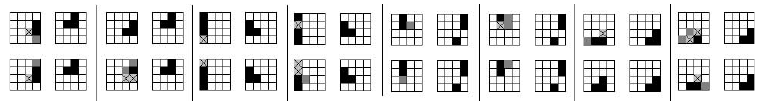
\includegraphics[width=0.98\textwidth]{img/datasets-k3.png} 
  \caption{BAL performance on \emph{CBVA}. Black color stands for target--estimate match, gray for target only and gray with a cross for false--positive estimate~\citep{farkas2013bal}.}
  \label{fig:datasets-k3}
\end{figure}

%tail -n +2 train.csv | sed 's/,/ /g' | awk 'BEGIN{FS=" "}{for(i=2;i<=NF;i++) {printf "%f ", $i / 256.0} printf "\n"}' >> buf.in
%echo "38000 784" > digits.in
%echo "4000 784" > digits.test.in
%tail -n +2 train.csv | sed 's/,/ /g' | awk 'BEGIN{FS=" "}{for(i=0;i<=9;i++) printf("%d ", $1 == i ? 1 : 0); printf "\n"}' > buf.out
%echo "38000 10" > digits.out
%echo "4000 10" > digits.test.out
%head -38000 buf.in >> digits.in 
%tail -4000 buf.in >> digits.test.in 
%head -38000 buf.out >> digits.out
%tail -4000 buf.out >> digits.test.out
%rm buf.* 
\subsubsection{Handwritten digits} 
\label{sec:datasets-digits} 

The well--known MNIST dataset of \emph{handwritten digits}~\citep{digits2014mnist} first analysed by~\citet{lecun1998gradient} consists of 42,000 $28 \times 28$ grayscale images mapped to ten classes each representing one digit. We have chosen this dataset for three reasons. First, it~is big and complex enough to test the practicallity of our models. Second, performance of many models is known on this dataset and therefore, we can easily compare performance of our models to these models. And third, we can easily visualize the backward \emph{blend} representations and intuitively see if our models perform well. These visualisations could be found in Section~\ref{sec:our-backward-repre}. 

\begin{figure}[H]
  \centering
  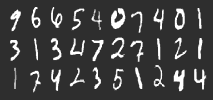
\includegraphics[width=0.4\textwidth]{img/digits.png} 
  \caption{Samples from the \emph{digits} dataset.}
  \label{fig:datasets-digits}
\end{figure}





\subsection{Evaluation methods} 
\label{sec:sim-evaluation} 

Following~\citet{farkas2013bal}, we measured two key properties of a BAL-like network. The more important being \emph{success rate} and second being \emph{convergence time}. 

\paragraph{Success rate.}  
Before comparing \emph{given} outputs on both visible layers the activations $Y^F$ and $X^B$ are classified by a treshold: 
\begin{equation} 
  g_k =
  \left\{
	  \begin{array}{ll}
		  1 & \mbox{if } x_k^B > 0.5 \\
		  0 & \mbox{otherwise}
	  \end{array}
  \right.  
\end{equation} 
By having a set of given vectors $G^I$ and the target vectors $T^I$ for inputs $I \in \mathbb{S}$, we distinguish two main success measures: 

%TODO remove itemize
\begin{itemize}
  \item \emph{Bit success (bitSucc)} defined as $bitSucc = avg_{I \in \mathbb{S}} \sum_i |T_i^I - G^I_i|$ and 
  \item \emph{Pattern success (patSucc)} defined as 
    \begin{equation}
      patSucc = avg_{I \in \mathbb{S}} \left\{
	      \begin{array}{ll}
		      1 & \mbox{if } T^I = G^I \\
		      0 & \mbox{otherwise}
	      \end{array}
      \right.
    \end{equation} 
\end{itemize} 

\paragraph{Convergence time.} The are several possibilities when to stop the learning algorithm. \emph{Converge time} is the number of epochs before the stop. Usually, training could be stopped for two reasons. The network could either reach the \emph{stopping criteria} or the maximum epoch is reached. Given by nature of used datasets we trained the neural networks while $patSucc^F \neq 1$. In case of the \emph{digits}~(\ref{sec:datasets-digits}) dataset we decided to stop the training if $patSucc^F$ was not increased for 3 epochs. Note that we are motivated to decrease the convergence time as it makes the training process faster.  
 

\newpage
    %Experimental Results and Analysis – in this section you should show the quantitative results – charts and tables. Analyze the results by explaining and highlighting what is important on them in terms of your goals and what is bad. You should explain the strange results too.

\section{Results and Analysis} 

\begin{figure}[t]
  \centering
  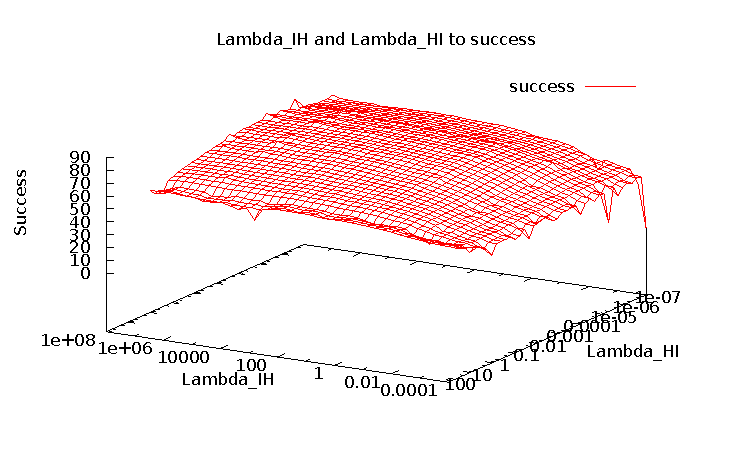
\includegraphics[width=0.8\textwidth]{img/success_to_lambdas.pdf}    
  \caption{Encoder 4-2-4: Performance of the two-lambda model with $\sigma = 2.3$ and $\mu = 0.0$.}
  \label{fig:424-success_to_lambdas}
\end{figure}
\begin{figure}[t]
  \centering
  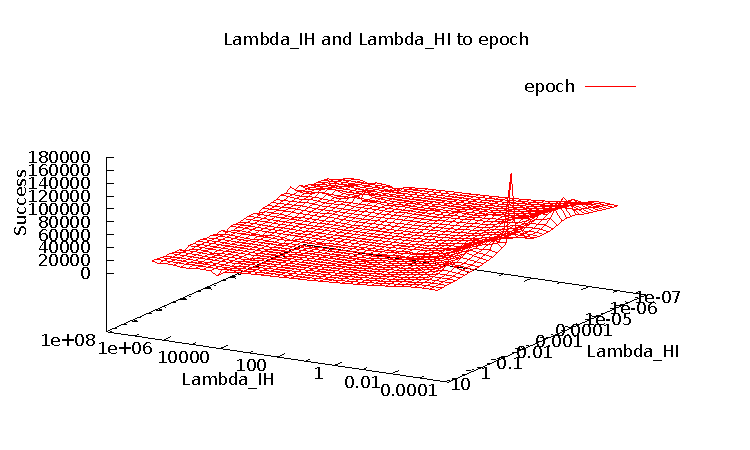
\includegraphics[width=0.8\textwidth]{img/epoch_to_lambdas.pdf}    
  \caption{Encoder 4-2-4: Convergence time of the two-lambda model with $\sigma = 2.3$ and $\mu = 0.0$.}
  \label{fig:424-epoch_to_lambdas}
\end{figure}

\begin{figure}[t]
  \centering
  \includegraphics[width=0.8\textwidth]{../bal/data/stats/test/epoch_to_err.pdf}    
  \caption{Encoder 4-2-4}
  \label{fig:424-test1}
\end{figure}


\begin{figure}[t]
  \centering
  \includegraphics[width=0.8\textwidth]{../bal/data/stats/test/epoch_to_h_dist.pdf}    
  \caption{Encoder 4-2-4}
  \label{fig:424-test2-1}
\end{figure}

% TODO forward backward error 
\begin{figure}[t]
  \centering
  \includegraphics[width=0.8\textwidth]{../bal/data/stats/test/epoch_to_success.pdf}    
  \caption{Encoder 4-2-4}
  \label{fig:424-test2-2}
\end{figure}

% TODO labels
% TODO compare several models 
\begin{figure}[t]
  \centering
  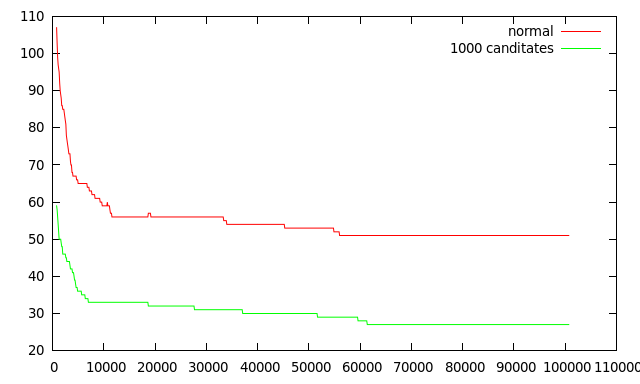
\includegraphics[width=0.8\textwidth]{../presentation/img/long_run_error.png}    
  \caption{Encoder 4-2-4 - Candidate selection vs. normal BAL}
  \label{fig:424-test2-3}
\end{figure}

% TODO hidden activation timelines (for each model) 
%\begin{figure}[t]
%  \centering
% 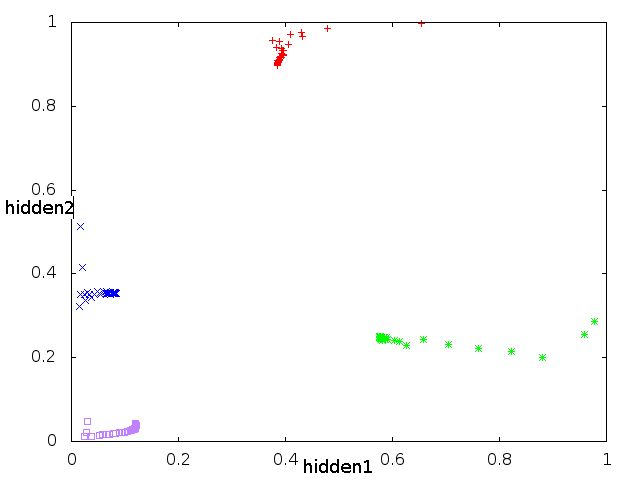
\includegraphics[width=0.8\textwidth]{../presentation/img/nice.png}    
%  \caption{Encoder 4-2-4 hidden activations - Nice}
%  \label{fig:424-test2}
%\end{figure}


\subsection{Comparison} 

TODO: success / learning rate 
TODO: epochs / learning rate 
TODO: success / epochs 
TODO: bitSucc and patSucc

TODO: success / hidden layer size 
\paragraph{Example k3:}
09-12-2013
\begin{itemize}  
\item 3  - 79.5\%
\item 4  - 94.9\%
\item 5  - 98.5\%
\item 6  - 99.5\%
\item 7  - 99.8\%
\item 8  - 99.9\%
\item 9  - 100.0\%
\item 10  - 100.0\%
\end{itemize} 

\paragraph{Example k12:}
TODO 

%TODO Mathematical analysis of the last model - o'really clanok aproximacia gradientu chyby
\subsection{Analysis} 
\begin{itemize} 
\item Matrices IH-OH and HO-HI tend to be same in autoassociative tasks. 
\item Hidden representation distance is a meaningful measure (LinReg on pre\_measure) (+ 10\%) . 
\item In triangle (non-convex). Not-in triangle is a must to condition for success. \\
TODO rerun to get "1 err in\_triangle" with and without preselection (there was a bug in the old data). 

\item Long run (+ 10\%). It seems it's always better to have long runs.  
\item reprezentacie na hidden absolutne rovnake (forward, backward), matice rozne:
\item Convergence Epsilon - weights tend to infinity (09-12-2013: Convergence which depends on average weight change does not work). 
\item Rerun - same config, different order when training 
All bad: \\
err sigma lambda momentum success sample\_ratio \\
0.0 2.3 0.7 0.0 19.296918767507005 6889/35700 \\
1.0 2.3 0.7 0.0 68.05602240896359 24296/35700 \\
2.0 2.3 0.7 0.0 12.644257703081232 4514/35700 \\
3.0 2.3 0.7 0.0 0.0028011204481792717 1/35700 \\

All good:  \\
err sigma lambda momentum success sample\_ratio \\
0.0 2.3 0.7 0.0 99.98911353032659 64293/64300 \\
1.0 2.3 0.7 0.0 0.01088646967340591 7/64300 \\

\end{itemize}

\subsubsection{Convergence} 
TODO make it shorter 

24-02-2014
TODO: Measure in how many cases the learning ends with convergence (no weight change) and divergence (oscialtion of seveal states). 

 Mathematical background on convergence and learning rule: 

(Hopfield networks, Wikipedia) The requirement that weights be symmetric is typically used, as it will guarantee that the energy function decreases monotonically while following the activation rules, and the network may exhibit some periodic or chaotic behaviour if non-symmetric weights are used. However, Hopfield found that this chaotic behavior is confined to relatively small parts of the phase space, and does not impair the network's ability to act as a content-addressable associative memory system.

(O'Reilly 1996) The GeneRec Approximation to AP BP
The analysis presented earlier in the paper shows that GeneRec should compute the same error derivatives as the Almeida-Pineda version of error backpropagation in a recurrent network if the following conditions hold:
  The difference of the plus and minus phase activation terms in GeneRec, which are updated in separate iterative activation settling phases, can be used to compute a unit’s error term instead of the iterative update of the difference itself, which is what Almeida-Pineda uses.
  The reciprocal weights are symmetric. This enables the activation signals from the output to the hidden units (via the recurrent weights) to reflect the contribution that the hidden units made to the output error (via the forward-going weights).
  The difference of activations in the plus and minus phases is a reasonable approximation to the difference of net inputs times the derivative of the sigmoidal activation function. Note that this only affects the overall magnitude of the weight derivatives, not their direction.
  
(PINnc89.pdf) 

\paragraph{Generec-Bias} 
Therefore we tried several settings: 
\begin{itemize} 
\item No bias - two patterns for 4-2-4, three patterns for 4-3-4, all four patterns for 4-4-4
\item Bias only on the input layer:  
4-2-4 best network error = 3.0 (tended to have two very profiled (0.95+, 0, 0, 0) and two very even (0.5, 0.5, 0.5, 0.5)  \\
4-3-4 about 75\% success rate 
\item Bias on both input and hidden layers: 
    4-2-4 0.0 1.0 0.5 0.1 91.74311926605505 100/109, almost no 1.0 errors 
          epochs ranged from 9 to 4500 \\ 
    4-3-4 about 100\% succes rate with about 20 epochs (epoch ranged from 5 to 700) 
\item Bias on all matrices (IH, HO, OH): 
    seems to add a little chaos with a slighty worse performance (but maybe bad sigma)

\end{itemize} 

$$r_x\frac{dx_i}{dt} = -x_i + \sum_j w_{ij} f(x_j) + I_i$$
TODO: Frome where comes this equation? 

There are several ways to guarantee convergence. One way is to
impose structure on the connectivity of the network, such as requiring
the weight matrix to be lower triangular or symmetric. Symmetry, al-
though mathematically elegant, is quite stringent because it constrains
microscopic connectivity by requiring pairs of neurons to be symmetri-
cally connected. A less stringent constraint is to require that the Jacobian
matrix be diagonally dominant. For equation (2.11, the Jacobian matrix
has the form: 

$$L_{ij} = \delta_{ij} - w_{ij}f'(x_j)$$
Guez et al. (1988) 

(PINnc89.pdf) then the gradient descent dynamics will not change the stability of the network. The need
for this assumption can be eliminated by choosing a dynamical system
which admits only stable behavior, even under learning, as was done by
Barhen et al. (1989). TODO look up Barhen et al. (1989) article 

TODO - general theorem concerning staiblity of networks with symmetric weights Cohen and Grossberg 1983 

GLOBAL ASYMPTOTIC STABILITY - the network will settle for any input 
FIXED POINT =similar= MEMORY

(pineda1987) Oscilation (on recurrent BP) could occur when substantial SELF-EXCITATION 

\subsubsection{High-dimensional data} 
TODO!! analysis of high-dimensional data (CBVA, HandWritten) 
It's not most relevant if only 4-2-4 was analysed. 

\subsection{TODO} 

\subsubsection{Measure - Weight decay}
A commonly-used bias or regularizing function is weight decay (e.g., Hinton, 1989a; Weigend et al., 1991).
We implemented two commonly-used forms of weight decay in the Bp and GeneRec networks, simple
weight decay and weight-elimination weight decay (Weigend et al., 1991). In simple weight decay, a con-
stant fraction of the weight value is subtracted at each weight update, and weight-elimination is similar
except that the rate of decay is a more complex function of the weight such that larger weights suffer rela-
tively less decay than smaller ones (supporting a prior assumption of a bimodal distribution of weight values
— one population of larger weights that are actually useful and another of near-zero weights that are not
useful; see Weigend et al., 1991 for details).
The results with these forms of weight decay for the 100 hidden unit network are shown in Figure 5.
Although a small amount (.002; smaller amounts had progressively smaller effects) of simple weight de-
cay appears to reliably improve generalization performance in both Bp and GeneRec, the difference is not
substantial. The weight-elimination version of weight decay always appears to impair, rather than improve,
performance. Although the specific forms of weight decay explored here were not overly successful in
this task, it is possible that other forms might perform better. Nevertheless, most forms of weight decay
\citet{o2001generalization} 

\subsubsection{Measure - Weight patterns} 
An examination of the weights in the trained networks clearly shows why generalization is impaired in the
interactive network (Figure 6). The units have not carved the input/output mapping into separable subsets
that can be independently combined for the novel testing items — instead, each unit participates in the
input/output mapping for multiple slots. Although this is true for both the backpropagation and GeneRec
networks, it is particularly damaging for the interactive GeneRec network because of its attractor dynamics.
In contrast, the feedforward backpropagation network is still capable of producing a roughly linear combi-
nation of hidden unit activations that yields reasonable (though far from perfect) levels of generalization. \citet{o2001generalization} 

Figure 7: Average pairwise overlap (normalized dot product or cosine) between hidden patterns corresponding to
inputs that differ by a) 75\% (1 out of 4 slots different) and b) 50\% (2 out of 4 slots different). Feedforward back-
propagation (Bp) remains much closer to a linear response level (75\% and 50\% hidden similarity, respectively) after
training compared to interactive GeneRec, which shows evidence of attractor dynamics pulling the network away from
a linear, combinatorial response to the inputs.

\subsubsection{Mathematics} 
\begin{itemize} 
\item dynamic systems 
\end{itemize}


    
% ==================== 16. Conclusion ========================
% This chapter should conclude on your contribution. It should highlight the key results from the research work. In this section, you should avoid mentioning new terms and statements not discussed throughout the main text. Also general aspects of the research work shouldn’t be repeated here. Conclusion shouldn’t be the abstract written in past tense. The conclusion should derive the important facts out of your work and results that you obtained.
\newpage
    % ==================== 16. Conclusion ========================
% This chapter should conclude on your contribution. It should highlight the key results from the research work. In this section, you should avoid mentioning new terms and statements not discussed throughout the main text. Also general aspects of the research work shouldn’t be repeated here. Conclusion shouldn’t be the abstract written in past tense. The conclusion should derive the important facts out of your work and results that you obtained.
%=== ZAVER ====
%\begin{itemize} 
%\item   toto je otvorene
%\item   toto vyzera tazko
%\item   tymto by sme sa zaoberali dalej (Future work) 
%\end{itemize} 

\section*{Conclusion}
\markboth{CONCLUSION}{}
\addcontentsline{toc}{section}{Conclusion}
\label{sec:conclusion} 

In our work, we proposed and analysed the Two learning rates (TLR) model, a modification of BAL, which increased the success rate from 62.7\% to 93.1\% on the 4-2-4 encoder task. We observed that BAL converges rapidly to the state, when the backward and forward activations converge to the same values. This has inspired our primary hypothesis to explain why BAL had problems learning the 4-2-4 encoder task. Our hypothesis was further confirmed by candidate selection, which selected the network with more distant hidden activations. This increased the success rate from 93.1\% to 99.84\% and reduced the number of epochs needed for convergence from 5845 to 150. Then we applied TLR on the handwritten digit recognition task using the architecture 784--300--10. Although TLR still has a performance gap compared to backpropagation, it achieved far better success rate than original BAL. %(TODO sim) 

We experimented with many different modifications of BAL, notably BAL-recirc, other GeneRec learning rules, dropout and multilayer GeneRec, but these did not prove to be useful. Standard modifications, such as batch training mode or adding momentum, showed no tendency in increasing the success rate of TLR. We admit that there is a space for improvement on these approaches.

\label{sec:future-work}
%What left unfinished from your work? What are you future plans to develop better your work?
Our work opened several ways to continue the analysis of BAL. For instance, it would be possible to predict success rate from the initial weights, as discussed in section~\ref{sec:our-weight-init-class}. Another option is to use four learning rates, one for each matrix, or dynamic learning rates for each connection as outlined in section~\ref{sec:our-dynamic-lambda}. Furthermore, we recommend analysing backward activations which showed counterintuitive behaviour in figure~\ref{fig:results-tlr-auto4-epoch}. Finally, TLR introduced one more parameter to the network setup and therefore a method for finding best pair learning rates would be usefull. 

%TODO candidate selection TDM 
%TODO symmetric BAL 


    
% ==================== 17. Future Work ========================
%What left unfinished from your work? What are you future plans to develop better your work?
%\newpage
%    %What left unfinished from your work? What are you future plans to develop better your work?

\section*{Future Work} 
Weight initialization: train on the dataset (initial weights + success). 

Analyse convergence 
(TODO ref hidden activations) \ref{sec:convergence} 

Weight decay: 
\ref{sec:weight-decay} 

Recirc close weight: 
\begin{equation}
o_k = \alpha t_k + (1-\alpha)f(\eta_k). 
\end{equation} 

Try TLR also with GeneRec (and BP?).  \\ 


Dynamic learning rate \ref{sec:our-dynamic-lambda}. 

Tricks with BP \citep{lecun2012efficient}. 

%    \label{future-work} 

% ==================== 18. Bibliography ========================
%Put a list of references.
\newpage
    %Put a list of references.
%TODO more citations 

\renewcommand{\refname}{Bibliography}
\phantomsection
\addcontentsline{toc}{section}{Bibliography}

\bibliographystyle{abbrv}
\bibliography{main}


    
% ==================== 19. Assignment ========================
%At the end of your thesis you can attach resources such as source code (or something like ASCII code table) that would improve the completeness of your thesis.
\newpage
    %At the end of your thesis you can attach resources such as source code (or something like ASCII code table) that would improve the completeness of your thesis.

\section*{Appendix A - Implementation}
\appendix
\addcontentsline{toc}{section}{Appendix A - Implementation}
\markboth{Appendix A}{}

%TODO crucial parts of the implementation 
%TODO additional tables, measures 

%Implementation – in implementation section you should mention the tools that you use to implement, the target environment (e.g. linux, windows). Limitations (e.g. buffer sizes, connections number).

\subsection{GeneRec} 
\label{sec:appendix-impl-generec} 

Activation is computed as in \ref{eq:models-generec-activation}.

\subsubsection{Bias} 
%TODO reformulate
%TODO add more recent citations 
%TODO add results with / without bias 
%TODO parse references 
The use of such biases in neural networks has been discussed in the context of the fundamental bias/variance tradeoff \citet{geman1992neural}. This tradeoff emphasizes the fact that biases that are appropriate for the task can greatly facilitate learning and generalization by reducing the level of variance, where variance reflects the extent to which parameters are underconstrained by learning, and thus free to vary, causing random errors in generalization. These biases are also known as regularizers \citet{poggio1990networks}. However, inappropriate biases can obviously hurt performance by introducing systematic errors, such that there is no such thing as a single universally beneficial set of biases (Wolpert, 1996a; Wolpert, 1996b). 

\subsubsection{Fluctuation} 
\label{sec:generec-fluctuation}





\end{document}
